\documentclass[12pt,a4paper]{article}

% FONTS
\usepackage{microtype}
\usepackage{graphicx}  % to include figures (can also use other packages)
\usepackage{color}
\usepackage{fancyvrb}

% LAYOUT
\textheight=230mm
\textwidth=160mm
\oddsidemargin=7mm
\evensidemargin=-10mm
\topmargin=-10mm
\headsep=20mm
\columnsep=5mm
\addtolength{\belowcaptionskip}{0.5em}

\renewcommand{\textfraction}{0.01}
\renewcommand{\floatpagefraction}{0.99}
\renewcommand{\topfraction}{0.9}
\renewcommand{\bottomfraction}{0.9}


\setlength{\hoffset}{-2cm}
\setlength{\voffset}{-2cm}
% Page defaults ...
\topmargin=0.5cm
\oddsidemargin=2.5cm
\textwidth=16cm
\textheight=22cm
% Allow the page size to vary a bit ...
\raggedbottom
% To avoid Latex to be too fussy with line breaking ...
\sloppy

% MATH
\usepackage{amsmath} % Adds a large collection of math symbols
\usepackage{amssymb}
\usepackage{amsfonts}
\usepackage{upgreek} % Adds in support for greek letters in roman typeset

\usepackage{siunitx}
% Unit typesetting
\sisetup{
  detect-weight = true, 
  separate-uncertainty=true,
  uncertainty-separator = {\,},
  list-units = single
}

\usepackage{ifthen} % for conditional statements
\usepackage{xspace} % To avoid problems with missing or double spaces after predefined symbols
\newboolean{uprightparticles}
\setboolean{uprightparticles}{false} %True for upright particle symbols
%%% $Id: lhcb-symbols-def.tex 90362 2016-04-07 13:38:32Z pkoppenb $
%%% ======================================================================
%%% Purpose: Standard LHCb aliases
%%% Author: Originally Ulrik Egede, adapted by Tomasz Skwarnicki for templates,
%%% rewritten by Chris Parkes
%%% Maintainer : Ulrik Egede (2010 - 2012)
%%% Maintainer : Rolf Oldeman (2012 - 2014)
%%% =======================================================================

%%% To use this file outside the normal LHCb document environment, the
%%% following should be added in a preamble (before \begin{document}
%%%
%%%\usepackage{ifthen} 
%%%\newboolean{uprightparticles}
%%%\setboolean{uprightparticles}{false} %Set true for upright particle symbols
\usepackage{xspace} 
\usepackage{upgreek}

%%%%%%%%%%%%%%%%%%%%%%%%%%%%%%%%%%%%%%%%%%%%%%%%%%%%%%%%%%%%
%%%
%%% The following is to ensure that the template automatically can process
%%% this file.
%%%
%%% Add comments with at least three %%% preceding.
%%% Add new sections with one % preceding
%%% Add new subsections with two %% preceding
%%%%%%%%%%%%%%%%%%%%%%%%%%%%%%%%%%%%%%%%%%%%%%%%%%%%%%%%%%%%

%%%%%%%%%%%%%
% Experiments
%%%%%%%%%%%%%
\def\lhcb {\mbox{LHCb}\xspace}
\def\atlas  {\mbox{ATLAS}\xspace}
\def\cms    {\mbox{CMS}\xspace}
\def\alice  {\mbox{ALICE}\xspace}
\def\babar  {\mbox{BaBar}\xspace}
\def\belle  {\mbox{Belle}\xspace}
\def\cleo   {\mbox{CLEO}\xspace}
\def\cdf    {\mbox{CDF}\xspace}
\def\dzero  {\mbox{D0}\xspace}
\def\aleph  {\mbox{ALEPH}\xspace}
\def\delphi {\mbox{DELPHI}\xspace}
\def\opal   {\mbox{OPAL}\xspace}
\def\lthree {\mbox{L3}\xspace}
\def\sld    {\mbox{SLD}\xspace}
%%%\def\argus  {\mbox{ARGUS}\xspace}
%%%\def\uaone  {\mbox{UA1}\xspace}
%%%\def\uatwo  {\mbox{UA2}\xspace}
%%%\def\ux85 {\mbox{UX85}\xspace}
\def\cern {\mbox{CERN}\xspace}
\def\lhc    {\mbox{LHC}\xspace}
\def\lep    {\mbox{LEP}\xspace}
\def\tevatron {Tevatron\xspace}

%% LHCb sub-detectors and sub-systems

%%%\def\pu     {PU\xspace}
\def\velo   {VELO\xspace}
\def\rich   {RICH\xspace}
\def\richone {RICH1\xspace}
\def\richtwo {RICH2\xspace}
\def\ttracker {TT\xspace}
\def\intr   {IT\xspace}
\def\st     {ST\xspace}
\def\ot     {OT\xspace}
%%%\def\Tone   {T1\xspace}
%%%\def\Ttwo   {T2\xspace}
%%%\def\Tthree {T3\xspace}
%%%\def\Mone   {M1\xspace}
%%%\def\Mtwo   {M2\xspace}
%%%\def\Mthree {M3\xspace}
%%%\def\Mfour  {M4\xspace}
%%%\def\Mfive  {M5\xspace}
\def\spd    {SPD\xspace}
\def\presh  {PS\xspace}
\def\ecal   {ECAL\xspace}
\def\hcal   {HCAL\xspace}
%%%\def\bcm    {BCM\xspace}
\def\MagUp {\mbox{\em Mag\kern -0.05em Up}\xspace}
\def\MagDown {\mbox{\em MagDown}\xspace}

\def\ode    {ODE\xspace}
\def\daq    {DAQ\xspace}
\def\tfc    {TFC\xspace}
\def\ecs    {ECS\xspace}
\def\lone   {L0\xspace}
\def\hlt    {HLT\xspace}
\def\hltone {HLT1\xspace}
\def\hlttwo {HLT2\xspace}

%%% Upright (not slanted) Particles

\ifthenelse{\boolean{uprightparticles}}%
{\def\Palpha      {\ensuremath{\upalpha}\xspace}
 \def\Pbeta       {\ensuremath{\upbeta}\xspace}
 \def\Pgamma      {\ensuremath{\upgamma}\xspace}                 
 \def\Pdelta      {\ensuremath{\updelta}\xspace}                 
 \def\Pepsilon    {\ensuremath{\upepsilon}\xspace}                 
 \def\Pvarepsilon {\ensuremath{\upvarepsilon}\xspace}                 
 \def\Pzeta       {\ensuremath{\upzeta}\xspace}                 
 \def\Peta        {\ensuremath{\upeta}\xspace}                 
 \def\Ptheta      {\ensuremath{\uptheta}\xspace}                 
 \def\Pvartheta   {\ensuremath{\upvartheta}\xspace}                 
 \def\Piota       {\ensuremath{\upiota}\xspace}                 
 \def\Pkappa      {\ensuremath{\upkappa}\xspace}                 
 \def\Plambda     {\ensuremath{\uplambda}\xspace}                 
 \def\Pmu         {\ensuremath{\upmu}\xspace}                 
 \def\Pnu         {\ensuremath{\upnu}\xspace}                 
 \def\Pxi         {\ensuremath{\upxi}\xspace}                 
 \def\Ppi         {\ensuremath{\uppi}\xspace}                 
 \def\Pvarpi      {\ensuremath{\upvarpi}\xspace}                 
 \def\Prho        {\ensuremath{\uprho}\xspace}                 
 \def\Pvarrho     {\ensuremath{\upvarrho}\xspace}                 
 \def\Ptau        {\ensuremath{\uptau}\xspace}                 
 \def\Pupsilon    {\ensuremath{\upupsilon}\xspace}                 
 \def\Pphi        {\ensuremath{\upphi}\xspace}                 
 \def\Pvarphi     {\ensuremath{\upvarphi}\xspace}                 
 \def\Pchi        {\ensuremath{\upchi}\xspace}                 
 \def\Ppsi        {\ensuremath{\uppsi}\xspace}                 
 \def\Pomega      {\ensuremath{\upomega}\xspace}                 

 \def\PDelta      {\ensuremath{\Delta}\xspace}                 
 \def\PXi      {\ensuremath{\Xi}\xspace}                 
 \def\PLambda      {\ensuremath{\Lambda}\xspace}                 
 \def\PSigma      {\ensuremath{\Sigma}\xspace}                 
 \def\POmega      {\ensuremath{\Omega}\xspace}                 
 \def\PUpsilon      {\ensuremath{\Upsilon}\xspace}                 
 
 %\mathchardef\Deltares="7101
 %\mathchardef\Xi="7104
 %\mathchardef\Lambda="7103
 %\mathchardef\Sigma="7106
 %\mathchardef\Omega="710A


 \def\PA      {\ensuremath{\mathrm{A}}\xspace}                 
 \def\PB      {\ensuremath{\mathrm{B}}\xspace}                 
 \def\PC      {\ensuremath{\mathrm{C}}\xspace}                 
 \def\PD      {\ensuremath{\mathrm{D}}\xspace}                 
 \def\PE      {\ensuremath{\mathrm{E}}\xspace}                 
 \def\PF      {\ensuremath{\mathrm{F}}\xspace}                 
 \def\PG      {\ensuremath{\mathrm{G}}\xspace}                 
 \def\PH      {\ensuremath{\mathrm{H}}\xspace}                 
 \def\PI      {\ensuremath{\mathrm{I}}\xspace}                 
 \def\PJ      {\ensuremath{\mathrm{J}}\xspace}                 
 \def\PK      {\ensuremath{\mathrm{K}}\xspace}                 
 \def\PL      {\ensuremath{\mathrm{L}}\xspace}                 
 \def\PM      {\ensuremath{\mathrm{M}}\xspace}                 
 \def\PN      {\ensuremath{\mathrm{N}}\xspace}                 
 \def\PO      {\ensuremath{\mathrm{O}}\xspace}                 
 \def\PP      {\ensuremath{\mathrm{P}}\xspace}                 
 \def\PQ      {\ensuremath{\mathrm{Q}}\xspace}                 
 \def\PR      {\ensuremath{\mathrm{R}}\xspace}                 
 \def\PS      {\ensuremath{\mathrm{S}}\xspace}                 
 \def\PT      {\ensuremath{\mathrm{T}}\xspace}                 
 \def\PU      {\ensuremath{\mathrm{U}}\xspace}                 
 \def\PV      {\ensuremath{\mathrm{V}}\xspace}                 
 \def\PW      {\ensuremath{\mathrm{W}}\xspace}                 
 \def\PX      {\ensuremath{\mathrm{X}}\xspace}                 
 \def\PY      {\ensuremath{\mathrm{Y}}\xspace}                 
 \def\PZ      {\ensuremath{\mathrm{Z}}\xspace}                 
 \def\Pa      {\ensuremath{\mathrm{a}}\xspace}                 
 \def\Pb      {\ensuremath{\mathrm{b}}\xspace}                 
 \def\Pc      {\ensuremath{\mathrm{c}}\xspace}                 
 \def\Pd      {\ensuremath{\mathrm{d}}\xspace}                 
 \def\Pe      {\ensuremath{\mathrm{e}}\xspace}                 
 \def\Pf      {\ensuremath{\mathrm{f}}\xspace}                 
 \def\Pg      {\ensuremath{\mathrm{g}}\xspace}                 
 \def\Ph      {\ensuremath{\mathrm{h}}\xspace}                 
 \def\Pi      {\ensuremath{\mathrm{i}}\xspace}                 
 \def\Pj      {\ensuremath{\mathrm{j}}\xspace}                 
 \def\Pk      {\ensuremath{\mathrm{k}}\xspace}                 
 \def\Pl      {\ensuremath{\mathrm{l}}\xspace}                 
 \def\Pm      {\ensuremath{\mathrm{m}}\xspace}                 
 \def\Pn      {\ensuremath{\mathrm{n}}\xspace}                 
 \def\Po      {\ensuremath{\mathrm{o}}\xspace}                 
 \def\Pp      {\ensuremath{\mathrm{p}}\xspace}                 
 \def\Pq      {\ensuremath{\mathrm{q}}\xspace}                 
 \def\Pr      {\ensuremath{\mathrm{r}}\xspace}                 
 \def\Ps      {\ensuremath{\mathrm{s}}\xspace}                 
 \def\Pt      {\ensuremath{\mathrm{t}}\xspace}                 
 \def\Pu      {\ensuremath{\mathrm{u}}\xspace}                 
 \def\Pv      {\ensuremath{\mathrm{v}}\xspace}                 
 \def\Pw      {\ensuremath{\mathrm{w}}\xspace}                 
 \def\Px      {\ensuremath{\mathrm{x}}\xspace}                 
 \def\Py      {\ensuremath{\mathrm{y}}\xspace}                 
 \def\Pz      {\ensuremath{\mathrm{z}}\xspace}                 
}
{\def\Palpha      {\ensuremath{\alpha}\xspace}
 \def\Pbeta       {\ensuremath{\beta}\xspace}
 \def\Pgamma      {\ensuremath{\gamma}\xspace}                 
 \def\Pdelta      {\ensuremath{\delta}\xspace}                 
 \def\Pepsilon    {\ensuremath{\epsilon}\xspace}                 
 \def\Pvarepsilon {\ensuremath{\varepsilon}\xspace}                 
 \def\Pzeta       {\ensuremath{\zeta}\xspace}                 
 \def\Peta        {\ensuremath{\eta}\xspace}                 
 \def\Ptheta      {\ensuremath{\theta}\xspace}                 
 \def\Pvartheta   {\ensuremath{\vartheta}\xspace}                 
 \def\Piota       {\ensuremath{\iota}\xspace}                 
 \def\Pkappa      {\ensuremath{\kappa}\xspace}                 
 \def\Plambda     {\ensuremath{\lambda}\xspace}                 
 \def\Pmu         {\ensuremath{\mu}\xspace}                 
 \def\Pnu         {\ensuremath{\nu}\xspace}                 
 \def\Pxi         {\ensuremath{\xi}\xspace}                 
 \def\Ppi         {\ensuremath{\pi}\xspace}                 
 \def\Pvarpi      {\ensuremath{\varpi}\xspace}                 
 \def\Prho        {\ensuremath{\rho}\xspace}                 
 \def\Pvarrho     {\ensuremath{\varrho}\xspace}                 
 \def\Ptau        {\ensuremath{\tau}\xspace}                 
 \def\Pupsilon    {\ensuremath{\upsilon}\xspace}                 
 \def\Pphi        {\ensuremath{\phi}\xspace}                 
 \def\Pvarphi     {\ensuremath{\varphi}\xspace}                 
 \def\Pchi        {\ensuremath{\chi}\xspace}                 
 \def\Ppsi        {\ensuremath{\psi}\xspace}                 
 \def\Pomega      {\ensuremath{\omega}\xspace}                 
 \mathchardef\PDelta="7101
 \mathchardef\PXi="7104
 \mathchardef\PLambda="7103
 \mathchardef\PSigma="7106
 \mathchardef\POmega="710A
 \mathchardef\PUpsilon="7107
 \def\PA      {\ensuremath{A}\xspace}                 
 \def\PB      {\ensuremath{B}\xspace}                 
 \def\PC      {\ensuremath{C}\xspace}                 
 \def\PD      {\ensuremath{D}\xspace}                 
 \def\PE      {\ensuremath{E}\xspace}                 
 \def\PF      {\ensuremath{F}\xspace}                 
 \def\PG      {\ensuremath{G}\xspace}                 
 \def\PH      {\ensuremath{H}\xspace}                 
 \def\PI      {\ensuremath{I}\xspace}                 
 \def\PJ      {\ensuremath{J}\xspace}                 
 \def\PK      {\ensuremath{K}\xspace}                 
 \def\PL      {\ensuremath{L}\xspace}                 
 \def\PM      {\ensuremath{M}\xspace}                 
 \def\PN      {\ensuremath{N}\xspace}                 
 \def\PO      {\ensuremath{O}\xspace}                 
 \def\PP      {\ensuremath{P}\xspace}                 
 \def\PQ      {\ensuremath{Q}\xspace}                 
 \def\PR      {\ensuremath{R}\xspace}                 
 \def\PS      {\ensuremath{S}\xspace}                 
 \def\PT      {\ensuremath{T}\xspace}                 
 \def\PU      {\ensuremath{U}\xspace}                 
 \def\PV      {\ensuremath{V}\xspace}                 
 \def\PW      {\ensuremath{W}\xspace}                 
 \def\PX      {\ensuremath{X}\xspace}                 
 \def\PY      {\ensuremath{Y}\xspace}                 
 \def\PZ      {\ensuremath{Z}\xspace}                 
 \def\Pa      {\ensuremath{a}\xspace}                 
 \def\Pb      {\ensuremath{b}\xspace}                 
 \def\Pc      {\ensuremath{c}\xspace}                 
 \def\Pd      {\ensuremath{d}\xspace}                 
 \def\Pe      {\ensuremath{e}\xspace}                 
 \def\Pf      {\ensuremath{f}\xspace}                 
 \def\Pg      {\ensuremath{g}\xspace}                 
 \def\Ph      {\ensuremath{h}\xspace}                 
 \def\Pi      {\ensuremath{i}\xspace}                 
 \def\Pj      {\ensuremath{j}\xspace}                 
 \def\Pk      {\ensuremath{k}\xspace}                 
 \def\Pl      {\ensuremath{l}\xspace}                 
 \def\Pm      {\ensuremath{m}\xspace}                 
 \def\Pn      {\ensuremath{n}\xspace}                 
 \def\Po      {\ensuremath{o}\xspace}                 
 \def\Pp      {\ensuremath{p}\xspace}                 
 \def\Pq      {\ensuremath{q}\xspace}                 
 \def\Pr      {\ensuremath{r}\xspace}                 
 \def\Ps      {\ensuremath{s}\xspace}                 
 \def\Pt      {\ensuremath{t}\xspace}                 
 \def\Pu      {\ensuremath{u}\xspace}                 
 \def\Pv      {\ensuremath{v}\xspace}                 
 \def\Pw      {\ensuremath{w}\xspace}                 
 \def\Px      {\ensuremath{x}\xspace}                 
 \def\Py      {\ensuremath{y}\xspace}                 
 \def\Pz      {\ensuremath{z}\xspace}                 
}

%%%%%%%%%%%%%%%%%%%%%%%%%%%%%%%%%%%%%%%%%%%%%%%
% Particles
\makeatletter
\ifcase \@ptsize \relax% 10pt
  \newcommand{\miniscule}{\@setfontsize\miniscule{4}{5}}% \tiny: 5/6
\or% 11pt
  \newcommand{\miniscule}{\@setfontsize\miniscule{5}{6}}% \tiny: 6/7
\or% 12pt
  \newcommand{\miniscule}{\@setfontsize\miniscule{5}{6}}% \tiny: 6/7
\fi
\makeatother


\DeclareRobustCommand{\optbar}[1]{\shortstack{{\miniscule (\rule[.5ex]{1.25em}{.18mm})}
  \\ [-.7ex] $#1$}}


%% Leptons

\let\emi\en
\def\electron   {{\ensuremath{\Pe}}\xspace}
\def\en         {{\ensuremath{\Pe^-}}\xspace}   % electron negative (\em is taken)
\def\ep         {{\ensuremath{\Pe^+}}\xspace}
\def\epm        {{\ensuremath{\Pe^\pm}}\xspace} 
\def\epem       {{\ensuremath{\Pe^+\Pe^-}}\xspace}
%%%\def\ee         {\ensuremath{\Pe^-\Pe^-}\xspace}

\def\muon       {{\ensuremath{\Pmu}}\xspace}
\def\mup        {{\ensuremath{\Pmu^+}}\xspace}
\def\mun        {{\ensuremath{\Pmu^-}}\xspace} % muon negative (\mum is taken)
\def\mumu       {{\ensuremath{\Pmu^+\Pmu^-}}\xspace}

\def\tauon      {{\ensuremath{\Ptau}}\xspace}
\def\taup       {{\ensuremath{\Ptau^+}}\xspace}
\def\taum       {{\ensuremath{\Ptau^-}}\xspace}
\def\tautau     {{\ensuremath{\Ptau^+\Ptau^-}}\xspace}

\def\lepton     {{\ensuremath{\ell}}\xspace}
\def\ellm       {{\ensuremath{\ell^-}}\xspace}
\def\ellp       {{\ensuremath{\ell^+}}\xspace}
\def\ellell     {\ensuremath{\ell^+ \ell^-}\xspace}

\def\neu        {{\ensuremath{\Pnu}}\xspace}
\def\neub       {{\ensuremath{\overline{\Pnu}}}\xspace}
%%%\def\nuenueb    {\ensuremath{\neu\neub}\xspace}
\def\neue       {{\ensuremath{\neu_e}}\xspace}
\def\neueb      {{\ensuremath{\neub_e}}\xspace}
%%%\def\neueneueb  {\ensuremath{\neue\neueb}\xspace}
\def\neum       {{\ensuremath{\neu_\mu}}\xspace}
\def\neumb      {{\ensuremath{\neub_\mu}}\xspace}
%%%\def\neumneumb  {\ensuremath{\neum\neumb}\xspace}
\def\neut       {{\ensuremath{\neu_\tau}}\xspace}
\def\neutb      {{\ensuremath{\neub_\tau}}\xspace}
%%%\def\neutneutb  {\ensuremath{\neut\neutb}\xspace}
\def\neul       {{\ensuremath{\neu_\ell}}\xspace}
\def\neulb      {{\ensuremath{\neub_\ell}}\xspace}
%%%\def\neulneulb  {\ensuremath{\neul\neulb}\xspace}

%% Gauge bosons and scalars

\def\g      {{\ensuremath{\Pgamma}}\xspace}
\def\H      {{\ensuremath{\PH^0}}\xspace}
\def\Hp     {{\ensuremath{\PH^+}}\xspace}
\def\Hm     {{\ensuremath{\PH^-}}\xspace}
\def\Hpm    {{\ensuremath{\PH^\pm}}\xspace}
\def\W      {{\ensuremath{\PW}}\xspace}
\def\Wp     {{\ensuremath{\PW^+}}\xspace}
\def\Wm     {{\ensuremath{\PW^-}}\xspace}
\def\Wpm    {{\ensuremath{\PW^\pm}}\xspace}
\def\Z      {{\ensuremath{\PZ}}\xspace}

%% Quarks

\def\quark     {{\ensuremath{\Pq}}\xspace}
\def\quarkbar  {{\ensuremath{\overline \quark}}\xspace}
\def\qqbar     {{\ensuremath{\quark\quarkbar}}\xspace}
\def\uquark    {{\ensuremath{\Pu}}\xspace}
\def\uquarkbar {{\ensuremath{\overline \uquark}}\xspace}
\def\uubar     {{\ensuremath{\uquark\uquarkbar}}\xspace}
\def\dquark    {{\ensuremath{\Pd}}\xspace}
\def\dquarkbar {{\ensuremath{\overline \dquark}}\xspace}
\def\ddbar     {{\ensuremath{\dquark\dquarkbar}}\xspace}
\def\squark    {{\ensuremath{\Ps}}\xspace}
\def\squarkbar {{\ensuremath{\overline \squark}}\xspace}
\def\ssbar     {{\ensuremath{\squark\squarkbar}}\xspace}
\def\cquark    {{\ensuremath{\Pc}}\xspace}
\def\cquarkbar {{\ensuremath{\overline \cquark}}\xspace}
\def\ccbar     {{\ensuremath{\cquark\cquarkbar}}\xspace}
\def\bquark    {{\ensuremath{\Pb}}\xspace}
\def\bquarkbar {{\ensuremath{\overline \bquark}}\xspace}
\def\bbbar     {{\ensuremath{\bquark\bquarkbar}}\xspace}
\def\tquark    {{\ensuremath{\Pt}}\xspace}
\def\tquarkbar {{\ensuremath{\overline \tquark}}\xspace}
\def\ttbar     {{\ensuremath{\tquark\tquarkbar}}\xspace}

%% Light mesons

\def\hadron {{\ensuremath{\Ph}}\xspace}
\def\pion   {{\ensuremath{\Ppi}}\xspace}
\def\piz    {{\ensuremath{\pion^0}}\xspace}
\def\pizs   {{\ensuremath{\pion^0\mbox\,\mathrm{s}}}\xspace}
\def\pip    {{\ensuremath{\pion^+}}\xspace}
\def\pim    {{\ensuremath{\pion^-}}\xspace}
\def\pipm   {{\ensuremath{\pion^\pm}}\xspace}
\def\pimp   {{\ensuremath{\pion^\mp}}\xspace}

\def\rhomeson {{\ensuremath{\Prho}}\xspace}
\def\rhoz     {{\ensuremath{\rhomeson^0}}\xspace}
\def\rhop     {{\ensuremath{\rhomeson^+}}\xspace}
\def\rhom     {{\ensuremath{\rhomeson^-}}\xspace}
\def\rhopm    {{\ensuremath{\rhomeson^\pm}}\xspace}
\def\rhomp    {{\ensuremath{\rhomeson^\mp}}\xspace}

\def\kaon    {{\ensuremath{\PK}}\xspace}
%%% do NOT use ensuremath here
  \def\Kbar    {{\kern 0.2em\overline{\kern -0.2em \PK}{}}\xspace}
\def\Kb      {{\ensuremath{\Kbar}}\xspace}
\def\KorKbar    {\kern 0.18em\optbar{\kern -0.18em K}{}\xspace}
\def\Kz      {{\ensuremath{\kaon^0}}\xspace}
\def\Kzb     {{\ensuremath{\Kbar{}^0}}\xspace}
\def\Kp      {{\ensuremath{\kaon^+}}\xspace}
\def\Km      {{\ensuremath{\kaon^-}}\xspace}
\def\Kpm     {{\ensuremath{\kaon^\pm}}\xspace}
\def\Kmp     {{\ensuremath{\kaon^\mp}}\xspace}
\def\KS      {{\ensuremath{\kaon^0_{\mathrm{ \scriptscriptstyle S}}}}\xspace}
\def\KL      {{\ensuremath{\kaon^0_{\mathrm{ \scriptscriptstyle L}}}}\xspace}
\def\Kstarz  {{\ensuremath{\kaon^{*0}}}\xspace}
\def\Kstarzb {{\ensuremath{\Kbar{}^{*0}}}\xspace}
\def\Kstar   {{\ensuremath{\kaon^*}}\xspace}
\def\Kstarb  {{\ensuremath{\Kbar{}^*}}\xspace}
\def\Kstarp  {{\ensuremath{\kaon^{*+}}}\xspace}
\def\Kstarm  {{\ensuremath{\kaon^{*-}}}\xspace}
\def\Kstarpm {{\ensuremath{\kaon^{*\pm}}}\xspace}
\def\Kstarmp {{\ensuremath{\kaon^{*\mp}}}\xspace}

\newcommand{\etaz}{\ensuremath{\Peta}\xspace}
\newcommand{\etapr}{\ensuremath{\Peta^{\prime}}\xspace}
\newcommand{\phiz}{\ensuremath{\Pphi}\xspace}
\newcommand{\omegaz}{\ensuremath{\Pomega}\xspace}

%% Heavy mesons

%%% do NOT use ensuremath here
  \def\Dbar    {{\kern 0.2em\overline{\kern -0.2em \PD}{}}\xspace}
\def\D       {{\ensuremath{\PD}}\xspace}
\def\Db      {{\ensuremath{\Dbar}}\xspace}
\def\DorDbar    {\kern 0.18em\optbar{\kern -0.18em D}{}\xspace}
\def\Dz      {{\ensuremath{\D^0}}\xspace}
\def\Dzb     {{\ensuremath{\Dbar{}^0}}\xspace}
\def\Dp      {{\ensuremath{\D^+}}\xspace}
\def\Dm      {{\ensuremath{\D^-}}\xspace}
\def\Dpm     {{\ensuremath{\D^\pm}}\xspace}
\def\Dmp     {{\ensuremath{\D^\mp}}\xspace}
\def\Dstar   {{\ensuremath{\D^*}}\xspace}
\def\Dstarb  {{\ensuremath{\Dbar{}^*}}\xspace}
\def\Dstarz  {{\ensuremath{\D^{*0}}}\xspace}
\def\Dstarzb {{\ensuremath{\Dbar{}^{*0}}}\xspace}
\def\Dstarp  {{\ensuremath{\D^{*+}}}\xspace}
\def\Dstarm  {{\ensuremath{\D^{*-}}}\xspace}
\def\Dstarpm {{\ensuremath{\D^{*\pm}}}\xspace}
\def\Dstarmp {{\ensuremath{\D^{*\mp}}}\xspace}
\def\Ds      {{\ensuremath{\D^+_\squark}}\xspace}
\def\Dsp     {{\ensuremath{\D^+_\squark}}\xspace}
\def\Dsm     {{\ensuremath{\D^-_\squark}}\xspace}
\def\Dspm    {{\ensuremath{\D^{\pm}_\squark}}\xspace}
\def\Dsmp    {{\ensuremath{\D^{\mp}_\squark}}\xspace}
\def\Dss     {{\ensuremath{\D^{*+}_\squark}}\xspace}
\def\Dssp    {{\ensuremath{\D^{*+}_\squark}}\xspace}
\def\Dssm    {{\ensuremath{\D^{*-}_\squark}}\xspace}
\def\Dsspm   {{\ensuremath{\D^{*\pm}_\squark}}\xspace}
\def\Dssmp   {{\ensuremath{\D^{*\mp}_\squark}}\xspace}

\def\B       {{\ensuremath{\PB}}\xspace}
%%% do NOT use ensuremath here
\def\Bbar    {{\ensuremath{\kern 0.18em\overline{\kern -0.18em \PB}{}}}\xspace}
\def\Bb      {{\ensuremath{\Bbar}}\xspace}
\def\BorBbar    {\kern 0.18em\optbar{\kern -0.18em B}{}\xspace}
\def\Bz      {{\ensuremath{\B^0}}\xspace}
\def\Bzb     {{\ensuremath{\Bbar{}^0}}\xspace}
\def\Bu      {{\ensuremath{\B^+}}\xspace}
\def\Bub     {{\ensuremath{\B^-}}\xspace}
\def\Bp      {{\ensuremath{\Bu}}\xspace}
\def\Bm      {{\ensuremath{\Bub}}\xspace}
\def\Bpm     {{\ensuremath{\B^\pm}}\xspace}
\def\Bmp     {{\ensuremath{\B^\mp}}\xspace}
\def\Bd      {{\ensuremath{\B^0}}\xspace}
\def\Bs      {{\ensuremath{\B^0_\squark}}\xspace}
\def\Bsb     {{\ensuremath{\Bbar{}^0_\squark}}\xspace}
\def\Bdb     {{\ensuremath{\Bbar{}^0}}\xspace}
\def\Bc      {{\ensuremath{\B_\cquark^+}}\xspace}
\def\Bcp     {{\ensuremath{\B_\cquark^+}}\xspace}
\def\Bcm     {{\ensuremath{\B_\cquark^-}}\xspace}
\def\Bcpm    {{\ensuremath{\B_\cquark^\pm}}\xspace}

%% Onia

\def\jpsi     {{\ensuremath{{\PJ\mskip -3mu/\mskip -2mu\Ppsi\mskip 2mu}}}\xspace}
\def\psitwos  {{\ensuremath{\Ppsi{(2S)}}}\xspace}
\def\psiprpr  {{\ensuremath{\Ppsi(3770)}}\xspace}
\def\etac     {{\ensuremath{\Peta_\cquark}}\xspace}
\def\chiczero {{\ensuremath{\Pchi_{\cquark 0}}}\xspace}
\def\chicone  {{\ensuremath{\Pchi_{\cquark 1}}}\xspace}
\def\chictwo  {{\ensuremath{\Pchi_{\cquark 2}}}\xspace}
  %\mathchardef\Upsilon="7107
  \def\Y#1S{\ensuremath{\PUpsilon{(#1S)}}\xspace}% no space before {...}!
\def\OneS  {{\Y1S}}
\def\TwoS  {{\Y2S}}
\def\ThreeS{{\Y3S}}
\def\FourS {{\Y4S}}
\def\FiveS {{\Y5S}}

\def\chic  {{\ensuremath{\Pchi_{c}}}\xspace}

%% Baryons

\def\proton      {{\ensuremath{\Pp}}\xspace}
\def\antiproton  {{\ensuremath{\overline \proton}}\xspace}
\def\neutron     {{\ensuremath{\Pn}}\xspace}
\def\antineutron {{\ensuremath{\overline \neutron}}\xspace}
\def\Deltares    {{\ensuremath{\PDelta}}\xspace}
\def\Deltaresbar {{\ensuremath{\overline \Deltares}}\xspace}
\def\Xires       {{\ensuremath{\PXi}}\xspace}
\def\Xiresbar    {{\ensuremath{\overline \Xires}}\xspace}
\def\Lz          {{\ensuremath{\PLambda}}\xspace}
\def\Lbar        {{\ensuremath{\kern 0.1em\overline{\kern -0.1em\PLambda}}}\xspace}
\def\LorLbar    {\kern 0.18em\optbar{\kern -0.18em \PLambda}{}\xspace}
\def\Lambdares   {{\ensuremath{\PLambda}}\xspace}
\def\Lambdaresbar{{\ensuremath{\Lbar}}\xspace}
\def\Sigmares    {{\ensuremath{\PSigma}}\xspace}
\def\Sigmaresbar {{\ensuremath{\overline \Sigmares}}\xspace}
\def\Omegares    {{\ensuremath{\POmega}}\xspace}
\def\Omegaresbar {{\ensuremath{\overline \POmega}}\xspace}

%%% do NOT use ensuremath here
 % \def\Deltabar{\kern 0.25em\overline{\kern -0.25em \Deltares}{}\xspace}
 % \def\Sigbar{\kern 0.2em\overline{\kern -0.2em \Sigma}{}\xspace}
 % \def\Xibar{\kern 0.2em\overline{\kern -0.2em \Xi}{}\xspace}
 % \def\Obar{\kern 0.2em\overline{\kern -0.2em \Omega}{}\xspace}
 % \def\Nbar{\kern 0.2em\overline{\kern -0.2em N}{}\xspace}
 % \def\Xb{\kern 0.2em\overline{\kern -0.2em X}{}\xspace}

\def\Lb      {{\ensuremath{\Lz^0_\bquark}}\xspace}
\def\Lbbar   {{\ensuremath{\Lbar{}^0_\bquark}}\xspace}
\def\Lc      {{\ensuremath{\Lz^+_\cquark}}\xspace}
\def\Lcbar   {{\ensuremath{\Lbar{}^-_\cquark}}\xspace}
\def\Xib     {{\ensuremath{\Xires_\bquark}}\xspace}
\def\Xibz    {{\ensuremath{\Xires^0_\bquark}}\xspace}
\def\Xibm    {{\ensuremath{\Xires^-_\bquark}}\xspace}
\def\Xibbar  {{\ensuremath{\Xiresbar{}_\bquark}}\xspace}
\def\Xibbarz {{\ensuremath{\Xiresbar{}_\bquark^0}}\xspace}
\def\Xibbarp {{\ensuremath{\Xiresbar{}_\bquark^+}}\xspace}
\def\Xic     {{\ensuremath{\Xires_\cquark}}\xspace}
\def\Xicz    {{\ensuremath{\Xires^0_\cquark}}\xspace}
\def\Xicp    {{\ensuremath{\Xires^+_\cquark}}\xspace}
\def\Xicbar  {{\ensuremath{\Xiresbar{}_\cquark}}\xspace}
\def\Xicbarz {{\ensuremath{\Xiresbar{}_\cquark^0}}\xspace}
\def\Xicbarm {{\ensuremath{\Xiresbar{}_\cquark^-}}\xspace}
\def\Omegac    {{\ensuremath{\Omegares^0_\cquark}}\xspace}
\def\Omegacbar {{\ensuremath{\Omegaresbar{}_\cquark^0}}\xspace}
\def\Omegab    {{\ensuremath{\Omegares^-_\bquark}}\xspace}
\def\Omegabbar {{\ensuremath{\Omegaresbar{}_\bquark^+}}\xspace}

%%%%%%%%%%%%%%%%%%
% Physics symbols
%%%%%%%%%%%%%%%%%

%% Decays
\def\BF         {{\ensuremath{\mathcal{B}}}\xspace}
\def\BRvis      {{\ensuremath{\BR_{\mathrm{{vis}}}}}}
\def\BR         {\BF}
\newcommand{\decay}[2]{\ensuremath{#1\!\to #2}\xspace}         % {\Pa}{\Pb \Pc}
\def\ra                 {\ensuremath{\rightarrow}\xspace}
\def\to                 {\ensuremath{\rightarrow}\xspace}

%% Lifetimes
\newcommand{\tauBs}{{\ensuremath{\tau_{\Bs}}}\xspace}
\newcommand{\tauBd}{{\ensuremath{\tau_{\Bd}}}\xspace}
\newcommand{\tauBz}{{\ensuremath{\tau_{\Bz}}}\xspace}
\newcommand{\tauBu}{{\ensuremath{\tau_{\Bp}}}\xspace}
\newcommand{\tauDp}{{\ensuremath{\tau_{\Dp}}}\xspace}
\newcommand{\tauDz}{{\ensuremath{\tau_{\Dz}}}\xspace}
\newcommand{\tauL}{{\ensuremath{\tau_{\mathrm{ L}}}}\xspace}
\newcommand{\tauH}{{\ensuremath{\tau_{\mathrm{ H}}}}\xspace}

%% Masses
\newcommand{\mBd}{{\ensuremath{m_{\Bd}}}\xspace}
\newcommand{\mBp}{{\ensuremath{m_{\Bp}}}\xspace}
\newcommand{\mBs}{{\ensuremath{m_{\Bs}}}\xspace}
\newcommand{\mBc}{{\ensuremath{m_{\Bc}}}\xspace}
\newcommand{\mLb}{{\ensuremath{m_{\Lb}}}\xspace}

%% EW theory, groups
\def\grpsuthree {{\ensuremath{\mathrm{SU}(3)}}\xspace}
\def\grpsutw    {{\ensuremath{\mathrm{SU}(2)}}\xspace}
\def\grpuone    {{\ensuremath{\mathrm{U}(1)}}\xspace}

\def\ssqtw   {{\ensuremath{\sin^{2}\!\theta_{\mathrm{W}}}}\xspace}
\def\csqtw   {{\ensuremath{\cos^{2}\!\theta_{\mathrm{W}}}}\xspace}
\def\stw     {{\ensuremath{\sin\theta_{\mathrm{W}}}}\xspace}
\def\ctw     {{\ensuremath{\cos\theta_{\mathrm{W}}}}\xspace}
\def\ssqtwef {{\ensuremath{{\sin}^{2}\theta_{\mathrm{W}}^{\mathrm{eff}}}}\xspace}
\def\csqtwef {{\ensuremath{{\cos}^{2}\theta_{\mathrm{W}}^{\mathrm{eff}}}}\xspace}
\def\stwef   {{\ensuremath{\sin\theta_{\mathrm{W}}^{\mathrm{eff}}}}\xspace}
\def\ctwef   {{\ensuremath{\cos\theta_{\mathrm{W}}^{\mathrm{eff}}}}\xspace}
\def\gv      {{\ensuremath{g_{\mbox{\tiny V}}}}\xspace}
\def\ga      {{\ensuremath{g_{\mbox{\tiny A}}}}\xspace}

\def\order   {{\ensuremath{\mathcal{O}}}\xspace}
\def\ordalph {{\ensuremath{\mathcal{O}(\alpha)}}\xspace}
\def\ordalsq {{\ensuremath{\mathcal{O}(\alpha^{2})}}\xspace}
\def\ordalcb {{\ensuremath{\mathcal{O}(\alpha^{3})}}\xspace}

%% QCD parameters
\newcommand{\as}{{\ensuremath{\alpha_s}}\xspace}
\newcommand{\MSb}{{\ensuremath{\overline{\mathrm{MS}}}}\xspace}
\newcommand{\lqcd}{{\ensuremath{\Lambda_{\mathrm{QCD}}}}\xspace}
\def\qsq       {{\ensuremath{q^2}}\xspace}

%% CKM, CP violation

\def\eps   {{\ensuremath{\varepsilon}}\xspace}
\def\epsK  {{\ensuremath{\varepsilon_K}}\xspace}
\def\epsB  {{\ensuremath{\varepsilon_B}}\xspace}
\def\epsp  {{\ensuremath{\varepsilon^\prime_K}}\xspace}

\def\CP                {{\ensuremath{C\!P}}\xspace}
\def\CPT               {{\ensuremath{C\!PT}}\xspace}

\def\rhobar {{\ensuremath{\overline \rho}}\xspace}
\def\etabar {{\ensuremath{\overline \eta}}\xspace}

\def\Vud  {{\ensuremath{V_{\uquark\dquark}}}\xspace}
\def\Vcd  {{\ensuremath{V_{\cquark\dquark}}}\xspace}
\def\Vtd  {{\ensuremath{V_{\tquark\dquark}}}\xspace}
\def\Vus  {{\ensuremath{V_{\uquark\squark}}}\xspace}
\def\Vcs  {{\ensuremath{V_{\cquark\squark}}}\xspace}
\def\Vts  {{\ensuremath{V_{\tquark\squark}}}\xspace}
\def\Vub  {{\ensuremath{V_{\uquark\bquark}}}\xspace}
\def\Vcb  {{\ensuremath{V_{\cquark\bquark}}}\xspace}
\def\Vtb  {{\ensuremath{V_{\tquark\bquark}}}\xspace}
\def\Vuds  {{\ensuremath{V_{\uquark\dquark}^\ast}}\xspace}
\def\Vcds  {{\ensuremath{V_{\cquark\dquark}^\ast}}\xspace}
\def\Vtds  {{\ensuremath{V_{\tquark\dquark}^\ast}}\xspace}
\def\Vuss  {{\ensuremath{V_{\uquark\squark}^\ast}}\xspace}
\def\Vcss  {{\ensuremath{V_{\cquark\squark}^\ast}}\xspace}
\def\Vtss  {{\ensuremath{V_{\tquark\squark}^\ast}}\xspace}
\def\Vubs  {{\ensuremath{V_{\uquark\bquark}^\ast}}\xspace}
\def\Vcbs  {{\ensuremath{V_{\cquark\bquark}^\ast}}\xspace}
\def\Vtbs  {{\ensuremath{V_{\tquark\bquark}^\ast}}\xspace}

%% Oscillations

\newcommand{\dm}{{\ensuremath{\Delta m}}\xspace}
\newcommand{\dms}{{\ensuremath{\Delta m_{\squark}}}\xspace}
\newcommand{\dmd}{{\ensuremath{\Delta m_{\dquark}}}\xspace}
\newcommand{\DG}{{\ensuremath{\Delta\Gamma}}\xspace}
\newcommand{\DGs}{{\ensuremath{\Delta\Gamma_{\squark}}}\xspace}
\newcommand{\DGd}{{\ensuremath{\Delta\Gamma_{\dquark}}}\xspace}
\newcommand{\Gs}{{\ensuremath{\Gamma_{\squark}}}\xspace}
\newcommand{\Gd}{{\ensuremath{\Gamma_{\dquark}}}\xspace}
\newcommand{\MBq}{{\ensuremath{M_{\B_\quark}}}\xspace}
\newcommand{\DGq}{{\ensuremath{\Delta\Gamma_{\quark}}}\xspace}
\newcommand{\Gq}{{\ensuremath{\Gamma_{\quark}}}\xspace}
\newcommand{\dmq}{{\ensuremath{\Delta m_{\quark}}}\xspace}
\newcommand{\GL}{{\ensuremath{\Gamma_{\mathrm{ L}}}}\xspace}
\newcommand{\GH}{{\ensuremath{\Gamma_{\mathrm{ H}}}}\xspace}
\newcommand{\DGsGs}{{\ensuremath{\Delta\Gamma_{\squark}/\Gamma_{\squark}}}\xspace}
\newcommand{\Delm}{{\mbox{$\Delta m $}}\xspace}
\newcommand{\ACP}{{\ensuremath{{\mathcal{A}}^{\CP}}}\xspace}
\newcommand{\Adir}{{\ensuremath{{\mathcal{A}}^{\mathrm{ dir}}}}\xspace}
\newcommand{\Amix}{{\ensuremath{{\mathcal{A}}^{\mathrm{ mix}}}}\xspace}
\newcommand{\ADelta}{{\ensuremath{{\mathcal{A}}^\Delta}}\xspace}
\newcommand{\phid}{{\ensuremath{\phi_{\dquark}}}\xspace}
\newcommand{\sinphid}{{\ensuremath{\sin\!\phid}}\xspace}
\newcommand{\phis}{{\ensuremath{\phi_{\squark}}}\xspace}
\newcommand{\betas}{{\ensuremath{\beta_{\squark}}}\xspace}
\newcommand{\sbetas}{{\ensuremath{\sigma(\beta_{\squark})}}\xspace}
\newcommand{\stbetas}{{\ensuremath{\sigma(2\beta_{\squark})}}\xspace}
\newcommand{\stphis}{{\ensuremath{\sigma(\phi_{\squark})}}\xspace}
\newcommand{\sinphis}{{\ensuremath{\sin\!\phis}}\xspace}

%% Tagging
\newcommand{\edet}{{\ensuremath{\varepsilon_{\mathrm{ det}}}}\xspace}
\newcommand{\erec}{{\ensuremath{\varepsilon_{\mathrm{ rec/det}}}}\xspace}
\newcommand{\esel}{{\ensuremath{\varepsilon_{\mathrm{ sel/rec}}}}\xspace}
\newcommand{\etrg}{{\ensuremath{\varepsilon_{\mathrm{ trg/sel}}}}\xspace}
\newcommand{\etot}{{\ensuremath{\varepsilon_{\mathrm{ tot}}}}\xspace}

\newcommand{\mistag}{\ensuremath{\omega}\xspace}
\newcommand{\wcomb}{\ensuremath{\omega^{\mathrm{comb}}}\xspace}
\newcommand{\etag}{{\ensuremath{\varepsilon_{\mathrm{tag}}}}\xspace}
\newcommand{\etagcomb}{{\ensuremath{\varepsilon_{\mathrm{tag}}^{\mathrm{comb}}}}\xspace}
\newcommand{\effeff}{\ensuremath{\varepsilon_{\mathrm{eff}}}\xspace}
\newcommand{\effeffcomb}{\ensuremath{\varepsilon_{\mathrm{eff}}^{\mathrm{comb}}}\xspace}
\newcommand{\efftag}{{\ensuremath{\etag(1-2\omega)^2}}\xspace}
\newcommand{\effD}{{\ensuremath{\etag D^2}}\xspace}

\newcommand{\etagprompt}{{\ensuremath{\varepsilon_{\mathrm{ tag}}^{\mathrm{Pr}}}}\xspace}
\newcommand{\etagLL}{{\ensuremath{\varepsilon_{\mathrm{ tag}}^{\mathrm{LL}}}}\xspace}

%% Key decay channels

\def\BdToKstmm    {\decay{\Bd}{\Kstarz\mup\mun}}
\def\BdbToKstmm   {\decay{\Bdb}{\Kstarzb\mup\mun}}

\def\BsToJPsiPhi  {\decay{\Bs}{\jpsi\phi}}
\def\BdToJPsiKst  {\decay{\Bd}{\jpsi\Kstarz}}
\def\BdbToJPsiKst {\decay{\Bdb}{\jpsi\Kstarzb}}

\def\BsPhiGam     {\decay{\Bs}{\phi \g}}
\def\BdKstGam     {\decay{\Bd}{\Kstarz \g}}

\def\BTohh        {\decay{\B}{\Ph^+ \Ph'^-}}
\def\BdTopipi     {\decay{\Bd}{\pip\pim}}
\def\BdToKpi      {\decay{\Bd}{\Kp\pim}}
\def\BsToKK       {\decay{\Bs}{\Kp\Km}}
\def\BsTopiK      {\decay{\Bs}{\pip\Km}}

%% Rare decays
\def\BdKstee  {\decay{\Bd}{\Kstarz\epem}}
\def\BdbKstee {\decay{\Bdb}{\Kstarzb\epem}}
\def\bsll     {\decay{\bquark}{\squark \ell^+ \ell^-}}
\def\AFB      {\ensuremath{A_{\mathrm{FB}}}\xspace}
\def\FL       {\ensuremath{F_{\mathrm{L}}}\xspace}
\def\AT#1     {\ensuremath{A_{\mathrm{T}}^{#1}}\xspace}           % 2
\def\btosgam  {\decay{\bquark}{\squark \g}}
\def\btodgam  {\decay{\bquark}{\dquark \g}}
\def\Bsmm     {\decay{\Bs}{\mup\mun}}
\def\Bdmm     {\decay{\Bd}{\mup\mun}}
\def\ctl       {\ensuremath{\cos{\theta_\ell}}\xspace}
\def\ctk       {\ensuremath{\cos{\theta_K}}\xspace}

%% Wilson coefficients and operators
\def\C#1      {\ensuremath{\mathcal{C}_{#1}}\xspace}                       % 9
\def\Cp#1     {\ensuremath{\mathcal{C}_{#1}^{'}}\xspace}                    % 7
\def\Ceff#1   {\ensuremath{\mathcal{C}_{#1}^{\mathrm{(eff)}}}\xspace}        % 9  
\def\Cpeff#1  {\ensuremath{\mathcal{C}_{#1}^{'\mathrm{(eff)}}}\xspace}       % 7
\def\Ope#1    {\ensuremath{\mathcal{O}_{#1}}\xspace}                       % 2
\def\Opep#1   {\ensuremath{\mathcal{O}_{#1}^{'}}\xspace}                    % 7

%% Charm

\def\xprime     {\ensuremath{x^{\prime}}\xspace}
\def\yprime     {\ensuremath{y^{\prime}}\xspace}
\def\ycp        {\ensuremath{y_{\CP}}\xspace}
\def\agamma     {\ensuremath{A_{\Gamma}}\xspace}
%%%\def\kpi        {\ensuremath{\PK\Ppi}\xspace}
%%%\def\kk         {\ensuremath{\PK\PK}\xspace}
%%%\def\dkpi       {\decay{\PD}{\PK\Ppi}}
%%%\def\dkk        {\decay{\PD}{\PK\PK}}
\def\dkpicf     {\decay{\Dz}{\Km\pip}}

%% QM
\newcommand{\bra}[1]{\ensuremath{\langle #1|}}             % {a}
\newcommand{\ket}[1]{\ensuremath{|#1\rangle}}              % {b}
\newcommand{\braket}[2]{\ensuremath{\langle #1|#2\rangle}} % {a}{b}

%%%%%%%%%%%%%%%%%%%%%%%%%%%%%%%%%%%%%%%%%%%%%%%%%%
% Units
%%%%%%%%%%%%%%%%%%%%%%%%%%%%%%%%%%%%%%%%%%%%%%%%%%
\newcommand{\unit}[1]{\ensuremath{\mathrm{ \,#1}}\xspace}          % {kg}

%% Energy and momentum
\newcommand{\tev}{\ifthenelse{\boolean{inbibliography}}{\ensuremath{~T\kern -0.05em eV}\xspace}{\ensuremath{\mathrm{\,Te\kern -0.1em V}}}\xspace}
\newcommand{\gev}{\ensuremath{\mathrm{\,Ge\kern -0.1em V}}\xspace}
\newcommand{\mev}{\ensuremath{\mathrm{\,Me\kern -0.1em V}}\xspace}
\newcommand{\kev}{\ensuremath{\mathrm{\,ke\kern -0.1em V}}\xspace}
\newcommand{\ev}{\ensuremath{\mathrm{\,e\kern -0.1em V}}\xspace}
\newcommand{\gevc}{\ensuremath{{\mathrm{\,Ge\kern -0.1em V\!/}c}}\xspace}
\newcommand{\mevc}{\ensuremath{{\mathrm{\,Me\kern -0.1em V\!/}c}}\xspace}
\newcommand{\gevcc}{\ensuremath{{\mathrm{\,Ge\kern -0.1em V\!/}c^2}}\xspace}
\newcommand{\gevgevcccc}{\ensuremath{{\mathrm{\,Ge\kern -0.1em V^2\!/}c^4}}\xspace}
\newcommand{\mevcc}{\ensuremath{{\mathrm{\,Me\kern -0.1em V\!/}c^2}}\xspace}

%% Distance and area
\def\km   {\ensuremath{\mathrm{ \,km}}\xspace}
\def\m    {\ensuremath{\mathrm{ \,m}}\xspace}
\def\ma   {\ensuremath{{\mathrm{ \,m}}^2}\xspace}
\def\cm   {\ensuremath{\mathrm{ \,cm}}\xspace}
\def\cma  {\ensuremath{{\mathrm{ \,cm}}^2}\xspace}
\def\mm   {\ensuremath{\mathrm{ \,mm}}\xspace}
\def\mma  {\ensuremath{{\mathrm{ \,mm}}^2}\xspace}
\def\mum  {\ensuremath{{\,\upmu\mathrm{m}}}\xspace}
\def\muma {\ensuremath{{\,\upmu\mathrm{m}^2}}\xspace}
\def\nm   {\ensuremath{\mathrm{ \,nm}}\xspace}
\def\fm   {\ensuremath{\mathrm{ \,fm}}\xspace}
\def\barn{\ensuremath{\mathrm{ \,b}}\xspace}
%%%\def\barnhyph{\ensuremath{\mathrm{ -b}}\xspace}
\def\mbarn{\ensuremath{\mathrm{ \,mb}}\xspace}
\def\mub{\ensuremath{{\mathrm{ \,\upmu b}}}\xspace}
%%%\def\mbarnhyph{\ensuremath{\mathrm{ -mb}}\xspace}
\def\nb {\ensuremath{\mathrm{ \,nb}}\xspace}
\def\invnb {\ensuremath{\mbox{\,nb}^{-1}}\xspace}
\def\pb {\ensuremath{\mathrm{ \,pb}}\xspace}
\def\invpb {\ensuremath{\mbox{\,pb}^{-1}}\xspace}
\def\fb   {\ensuremath{\mbox{\,fb}}\xspace}
\def\invfb   {\ensuremath{\mbox{\,fb}^{-1}}\xspace}
\def\ab   {\ensuremath{\mbox{\,ab}}\xspace}
\def\invab   {\ensuremath{\mbox{\,ab}^{-1}}\xspace}

%% Time 
\def\sec  {\ensuremath{\mathrm{{\,s}}}\xspace}
\def\ms   {\ensuremath{{\mathrm{ \,ms}}}\xspace}
\def\mus  {\ensuremath{{\,\upmu{\mathrm{ s}}}}\xspace}
\def\ns   {\ensuremath{{\mathrm{ \,ns}}}\xspace}
\def\ps   {\ensuremath{{\mathrm{ \,ps}}}\xspace}
\def\fs   {\ensuremath{\mathrm{ \,fs}}\xspace}

\def\mhz  {\ensuremath{{\mathrm{ \,MHz}}}\xspace}
\def\khz  {\ensuremath{{\mathrm{ \,kHz}}}\xspace}
\def\hz   {\ensuremath{{\mathrm{ \,Hz}}}\xspace}

\def\invps{\ensuremath{{\mathrm{ \,ps^{-1}}}}\xspace}
\def\invns{\ensuremath{{\mathrm{ \,ns^{-1}}}}\xspace}

\def\yr   {\ensuremath{\mathrm{ \,yr}}\xspace}
\def\hr   {\ensuremath{\mathrm{ \,hr}}\xspace}

%% Temperature
\def\degc {\ensuremath{^\circ}{C}\xspace}
\def\degk {\ensuremath {\mathrm{ K}}\xspace}

%% Material lengths, radiation
\def\Xrad {\ensuremath{X_0}\xspace}
\def\NIL{\ensuremath{\lambda_{int}}\xspace}
\def\mip {MIP\xspace}
\def\neutroneq {\ensuremath{\mathrm{ \,n_{eq}}}\xspace}
\def\neqcmcm {\ensuremath{\mathrm{ \,n_{eq} / cm^2}}\xspace}
\def\kRad {\ensuremath{\mathrm{ \,kRad}}\xspace}
\def\MRad {\ensuremath{\mathrm{ \,MRad}}\xspace}
\def\ci {\ensuremath{\mathrm{ \,Ci}}\xspace}
\def\mci {\ensuremath{\mathrm{ \,mCi}}\xspace}

%% Uncertainties
\def\sx    {\ensuremath{\sigma_x}\xspace}    
\def\sy    {\ensuremath{\sigma_y}\xspace}   
\def\sz    {\ensuremath{\sigma_z}\xspace}    

\newcommand{\stat}{\ensuremath{\mathrm{\,(stat)}}\xspace}
\newcommand{\syst}{\ensuremath{\mathrm{\,(syst)}}\xspace}

%% Maths

\def\order{{\ensuremath{\mathcal{O}}}\xspace}
\newcommand{\chisq}{\ensuremath{\chi^2}\xspace}
\newcommand{\chisqndf}{\ensuremath{\chi^2/\mathrm{ndf}}\xspace}
\newcommand{\chisqip}{\ensuremath{\chi^2_{\text{IP}}}\xspace}
\newcommand{\chisqvs}{\ensuremath{\chi^2_{\text{VS}}}\xspace}
\newcommand{\chisqvtx}{\ensuremath{\chi^2_{\text{vtx}}}\xspace}
\newcommand{\chisqvtxndf}{\ensuremath{\chi^2_{\text{vtx}}/\mathrm{ndf}}\xspace}

\def\deriv {\ensuremath{\mathrm{d}}}

\def\gsim{{~\raise.15em\hbox{$>$}\kern-.85em
          \lower.35em\hbox{$\sim$}~}\xspace}
\def\lsim{{~\raise.15em\hbox{$<$}\kern-.85em
          \lower.35em\hbox{$\sim$}~}\xspace}

\newcommand{\mean}[1]{\ensuremath{\left\langle #1 \right\rangle}} % {x}
\newcommand{\abs}[1]{\ensuremath{\left\|#1\right\|}} % {x}
\newcommand{\Real}{\ensuremath{\mathcal{R}e}\xspace}
\newcommand{\Imag}{\ensuremath{\mathcal{I}m}\xspace}

\def\PDF {PDF\xspace}

\def\sPlot{\mbox{\em sPlot}\xspace}
%%%\def\sWeight{\mbox{\em sWeight}\xspace}

%%%%%%%%%%%%%%%%%%%%%%%%%%%%%%%%%%%%%%%%%%%%%%%%%%
% Kinematics
%%%%%%%%%%%%%%%%%%%%%%%%%%%%%%%%%%%%%%%%%%%%%%%%%%

%% Energy, Momenta
\def\Ebeam {\ensuremath{E_{\mbox{\tiny BEAM}}}\xspace}
\def\sqs   {\ensuremath{\protect\sqrt{s}}\xspace}

\def\ptot       {\mbox{$p$}\xspace}
\def\pt         {\mbox{$p_{\mathrm{ T}}$}\xspace}
\def\et         {\mbox{$E_{\mathrm{ T}}$}\xspace}
\def\mt         {\mbox{$M_{\mathrm{ T}}$}\xspace}
\def\dpp        {\ensuremath{\Delta p/p}\xspace}
\def\msq        {\ensuremath{m^2}\xspace}
\newcommand{\dedx}{\ensuremath{\mathrm{d}\hspace{-0.1em}E/\mathrm{d}x}\xspace}

%% PID

\def\dllkpi     {\ensuremath{\mathrm{DLL}_{\kaon\pion}}\xspace}
\def\dllppi     {\ensuremath{\mathrm{DLL}_{\proton\pion}}\xspace}
\def\dllepi     {\ensuremath{\mathrm{DLL}_{\electron\pion}}\xspace}
\def\dllmupi    {\ensuremath{\mathrm{DLL}_{\muon\pi}}\xspace}

%% Geometry
%%%\def\mphi       {\mbox{$\phi$}\xspace}
%%%\def\mtheta     {\mbox{$\theta$}\xspace}
%%%\def\ctheta     {\mbox{$\cos\theta$}\xspace}
%%%\def\stheta     {\mbox{$\sin\theta$}\xspace}
%%%\def\ttheta     {\mbox{$\tan\theta$}\xspace}

\def\degrees{\ensuremath{^{\circ}}\xspace}
\def\krad {\ensuremath{\mathrm{ \,krad}}\xspace}
\def\mrad{\ensuremath{\mathrm{ \,mrad}}\xspace}
\def\rad{\ensuremath{\mathrm{ \,rad}}\xspace}

%% Accelerator
\def\betastar {\ensuremath{\beta^*}}
\newcommand{\lum} {\ensuremath{\mathcal{L}}\xspace}
\newcommand{\intlum}[1]{\ensuremath{\int\lum=#1}\xspace}  % {2 \,\invfb}

%%%%%%%%%%%%%%%%%%%%%%%%%%%%%%%%%%%%%%%%%%%%%%%%%%%%%%%%%%%%%%%%%%%%
% Software
%%%%%%%%%%%%%%%%%%%%%%%%%%%%%%%%%%%%%%%%%%%%%%%%%%%%%%%%%%%%%%%%%%%%

%% Programs
%%%\def\ansys      {\mbox{\textsc{Ansys}}\xspace}
\def\bcvegpy    {\mbox{\textsc{Bcvegpy}}\xspace}
\def\boole      {\mbox{\textsc{Boole}}\xspace}
\def\brunel     {\mbox{\textsc{Brunel}}\xspace}
\def\davinci    {\mbox{\textsc{DaVinci}}\xspace}
\def\dirac      {\mbox{\textsc{Dirac}}\xspace}
%%%\def\erasmus    {\mbox{\textsc{Erasmus}}\xspace}
\def\evtgen     {\mbox{\textsc{EvtGen}}\xspace}
\def\fewz       {\mbox{\textsc{Fewz}}\xspace}
\def\fluka      {\mbox{\textsc{Fluka}}\xspace}
\def\ganga      {\mbox{\textsc{Ganga}}\xspace}
%%%\def\garfield   {\mbox{\textsc{Garfield}}\xspace}
\def\gaudi      {\mbox{\textsc{Gaudi}}\xspace}
\def\gauss      {\mbox{\textsc{Gauss}}\xspace}
\def\geant      {\mbox{\textsc{Geant4}}\xspace}
\def\hepmc      {\mbox{\textsc{HepMC}}\xspace}
\def\herwig     {\mbox{\textsc{Herwig}}\xspace}
\def\moore      {\mbox{\textsc{Moore}}\xspace}
\def\neurobayes {\mbox{\textsc{NeuroBayes}}\xspace}
\def\photos     {\mbox{\textsc{Photos}}\xspace}
\def\powheg     {\mbox{\textsc{Powheg}}\xspace}
%%%\def\pyroot     {\mbox{\textsc{PyRoot}}\xspace}
\def\pythia     {\mbox{\textsc{Pythia}}\xspace}
\def\resbos     {\mbox{\textsc{ResBos}}\xspace}
\def\roofit     {\mbox{\textsc{RooFit}}\xspace}
\def\root       {\mbox{\textsc{Root}}\xspace}
\def\spice      {\mbox{\textsc{Spice}}\xspace}
%%%\def\tosca      {\mbox{\textsc{Tosca}}\xspace}
\def\urania     {\mbox{\textsc{Urania}}\xspace}

%% Languages
\def\cpp        {\mbox{\textsc{C\raisebox{0.1em}{{\footnotesize{++}}}}}\xspace}
%%%\def\python     {\mbox{\textsc{Python}}\xspace}
\def\ruby       {\mbox{\textsc{Ruby}}\xspace}
\def\fortran    {\mbox{\textsc{Fortran}}\xspace}
\def\svn        {\mbox{\textsc{SVN}}\xspace}

%% Data processing
\def\kbytes     {\ensuremath{{\mathrm{ \,kbytes}}}\xspace}
\def\kbsps      {\ensuremath{{\mathrm{ \,kbytes/s}}}\xspace}
\def\kbits      {\ensuremath{{\mathrm{ \,kbits}}}\xspace}
\def\kbsps      {\ensuremath{{\mathrm{ \,kbits/s}}}\xspace}
\def\mbsps      {\ensuremath{{\mathrm{ \,Mbits/s}}}\xspace}
\def\mbytes     {\ensuremath{{\mathrm{ \,Mbytes}}}\xspace}
\def\mbps       {\ensuremath{{\mathrm{ \,Mbyte/s}}}\xspace}
\def\mbsps      {\ensuremath{{\mathrm{ \,Mbytes/s}}}\xspace}
\def\gbsps      {\ensuremath{{\mathrm{ \,Gbits/s}}}\xspace}
\def\gbytes     {\ensuremath{{\mathrm{ \,Gbytes}}}\xspace}
\def\gbsps      {\ensuremath{{\mathrm{ \,Gbytes/s}}}\xspace}
\def\tbytes     {\ensuremath{{\mathrm{ \,Tbytes}}}\xspace}
\def\tbpy       {\ensuremath{{\mathrm{ \,Tbytes/yr}}}\xspace}

\def\dst        {DST\xspace}

%%%%%%%%%%%%%%%%%%%%%%%%%%%
% Detector related
%%%%%%%%%%%%%%%%%%%%%%%%%%%

%% Detector technologies
\def\nonn {\ensuremath{\mathrm{{ \mathit{n^+}} \mbox{-} on\mbox{-}{ \mathit{n}}}}\xspace}
\def\ponn {\ensuremath{\mathrm{{ \mathit{p^+}} \mbox{-} on\mbox{-}{ \mathit{n}}}}\xspace}
\def\nonp {\ensuremath{\mathrm{{ \mathit{n^+}} \mbox{-} on\mbox{-}{ \mathit{p}}}}\xspace}
\def\cvd  {CVD\xspace}
\def\mwpc {MWPC\xspace}
\def\gem  {GEM\xspace}

%% Detector components, electronics
\def\tell1  {TELL1\xspace}
\def\ukl1   {UKL1\xspace}
\def\beetle {Beetle\xspace}
\def\otis   {OTIS\xspace}
\def\croc   {CROC\xspace}
\def\carioca {CARIOCA\xspace}
\def\dialog {DIALOG\xspace}
\def\sync   {SYNC\xspace}
\def\cardiac {CARDIAC\xspace}
\def\gol    {GOL\xspace}
\def\vcsel  {VCSEL\xspace}
\def\ttc    {TTC\xspace}
\def\ttcrx  {TTCrx\xspace}
\def\hpd    {HPD\xspace}
\def\pmt    {PMT\xspace}
\def\specs  {SPECS\xspace}
\def\elmb   {ELMB\xspace}
\def\fpga   {FPGA\xspace}
\def\plc    {PLC\xspace}
\def\rasnik {RASNIK\xspace}
\def\elmb   {ELMB\xspace}
\def\can    {CAN\xspace}
\def\lvds   {LVDS\xspace}
\def\ntc    {NTC\xspace}
\def\adc    {ADC\xspace}
\def\led    {LED\xspace}
\def\ccd    {CCD\xspace}
\def\hv     {HV\xspace}
\def\lv     {LV\xspace}
\def\pvss   {PVSS\xspace}
\def\cmos   {CMOS\xspace}
\def\fifo   {FIFO\xspace}
\def\ccpc   {CCPC\xspace}

%% Chemical symbols
\def\cfourften     {\ensuremath{\mathrm{ C_4 F_{10}}}\xspace}
\def\cffour        {\ensuremath{\mathrm{ CF_4}}\xspace}
\def\cotwo         {\ensuremath{\mathrm{ CO_2}}\xspace} 
\def\csixffouteen  {\ensuremath{\mathrm{ C_6 F_{14}}}\xspace} 
\def\mgftwo     {\ensuremath{\mathrm{ Mg F_2}}\xspace} 
\def\siotwo     {\ensuremath{\mathrm{ SiO_2}}\xspace} 

%%%%%%%%%%%%%%%
% Special Text 
%%%%%%%%%%%%%%%
\newcommand{\eg}{\mbox{\itshape e.g.}\xspace}
\newcommand{\ie}{\mbox{\itshape i.e.}\xspace}
\newcommand{\etal}{\mbox{\itshape et al.}\xspace}
\newcommand{\etc}{\mbox{\itshape etc.}\xspace}
\newcommand{\cf}{\mbox{\itshape cf.}\xspace}
\newcommand{\ffp}{\mbox{\itshape ff.}\xspace}
\newcommand{\vs}{\mbox{\itshape vs.}\xspace}

%!TEX root = ../main.tex
%% JpsiKS specific
\def\BdToJPsiKS         {\ensuremath{\decay{\Bd}{J/\psi\KS}}\xspace}
\def\BsToJPsiKS         {\ensuremath{\decay{\Bs}{J/\psi\KS}}\xspace}
\def\BToJPsiKS          {\ensuremath{\decay{\PB}{J/\psi\KS}}\xspace}
\def\SJpsiKS            {\ensuremath{S_{J/\psi\KS}}\xspace}
\def\CJpsiKS            {\ensuremath{C_{J/\psi\KS}}\xspace}
\def\JPsiToMuMu         {\decay{J/\psi}{\mumu}}
\def\JPsiToee           {\decay{J/\psi}{\epem}}
\def\KSToPiPi           {\decay{\KS}{\pipi}}
\def\sintwobeta         {\ensuremath{\sin 2\beta}\xspace}

%% fixing Jpsi
\def\JpsiX              {\ensuremath{J/\psi\PX}\xspace}
\def\BdToJPsiKstar      {\ensuremath{\decay{\Bd}{J/\psi\Kstarz}}\xspace}
\def\BToJPsiKstar       {\ensuremath{\decay{\PB}{J/\psi\Kstar}}\xspace}
\def\BuToJPsiK          {\decay{\Bu}{J/\psi\Kp}}
\def\myBsToJPsiPhi      {\ensuremath{\decay{\Bs}{J/\psi\phi}}\xspace}
\def\BsToJPsiKst        {\decay{\Bs}{J/\psi\Kstarzb}}
\def\BuToJPsiPi         {\decay{\Bu}{J/\psi\pip}}
\def\BsToJPsiPiPi       {\decay{\Bs}{J/\psi\pipi}}
\def\BsToJPsiKK         {\decay{\Bs}{J/\psi\KpKm}}
\def\BsToJPsiPhiPhi     {\ensuremath{\decay{\Bs}{J/\psi\phi\phi}}\xspace}
\def\BsToJPsiFourhPhi   {\ensuremath{\decay{\Bs}{J/\psi(\to 4h)\phi}}\xspace}
\def\BsToJPsiF          {\ensuremath{\decay{\Bs}{J/\psi f_0(980)}}\xspace}
\def\BdToJPsiPiPi       {\ensuremath{\decay{\Bd}{J\psi\pipi}}\xspace}
\def\BdToJPsiX          {\ensuremath{\decay{\Bd}{J/\psi\PX}}\xspace}
\def\BuToJPsiX          {\ensuremath{\decay{\Bu}{J/\psi\PX}}\xspace}
\def\BsToJPsiX          {\ensuremath{\decay{\Bs}{J/\psi\PX}}\xspace}
\def\BdToJPsiRho        {\ensuremath{\decay{\Bd}{J/\psi\rho^{0}(770)}}\xspace}
\def\LbToJPsiL          {\ensuremath{\decay{\Lb}{J/\psi\Lz}}\xspace}

%% further decays from the B2CC WG
\def\BsToPsiTwoSKpi     {\decay{\Bsb}{\psitwos\Kp\pim}}
\def\BsToEtacPPbarPhi   {\ensuremath{\decay{\Bs}{\etac(\to\proton\antiproton)\phi}}\xspace}
\def\BsToEtacFourhPhi   {\ensuremath{\decay{\Bs}{\etac(\to 4h)\phi}}\xspace}
\def\BsToEtacPPbarPiPi  {\decay{\Bs}{\etac(\to\proton\antiproton)\pipi}}
\def\BsToEtacPPbarKK    {\ensuremath{\decay{\Bs}{\etac(\to\proton\antiproton)\KpKm}}\xspace}
\def\BsToEtacPhi        {\decay{\Bs}{\etac\phi}}
\def\BsToPsiTwoSPhi     {\ensuremath{\decay{\Bs}{\psitwos\phi}}\xspace}
\def\PhiToKK            {\ensuremath{\decay{\phi}{\KpKm}}\xspace}
\def\BsToChicPhi        {\ensuremath{\decay{\Bs}{\chiczero\phi}}\xspace}
\def\BToPsiKpi          {\ensuremath{\decay{\PB}{\psi K\pi}}\xspace}
\def\BdToPsiTwoSKS      {\ensuremath{\decay{\Bd}{\psitwos\KS}}\xspace}

%% B2OC specific decays
\def\allBToDD           {\ensuremath{\decay{\Bd}{\D^{(*)+}_{(\squark)}\D^{(*)-}}}\xspace}
\def\BdToDD             {\ensuremath{\decay{\Bd}{\Dp\Dm}}\xspace}
\def\BdToDDlegend       {\ensuremath{\decay{\B^0_{}}{\Dp\Dm}}\xspace}
\def\BsToDD             {\ensuremath{\decay{\Bs}{\Dp\Dm}}\xspace}
\def\BToDD              {\ensuremath{\decay{\PB}{\Dp\Dm}}\xspace}
\def\BToDDbar           {\ensuremath{\decay{\PB}{\D\Dbar}}\xspace}
\def\BdToDstDst         {\ensuremath{\decay{\Bd}{\Dstarp\Dstarm}}\xspace}
\def\BdToDsD            {\ensuremath{\decay{\Bd}{\Dsp\Dm}}\xspace}
\def\BsToDsD            {\ensuremath{\decay{\Bs}{\Dsm\Dp}}\xspace}
\def\BToDsD             {\ensuremath{\decay{\PB}{\D_\squark\PD}}\xspace}
\def\BdToDstD           {\ensuremath{\decay{\Bd}{\Dstarp\Dm}}\xspace}
\def\BsToDstD           {\ensuremath{\decay{\Bs}{\Dstarp\Dm}}\xspace}
\def\BToDstD            {\ensuremath{\decay{\PB}{\Dstarp\Dm}}\xspace}
\def\BsToDstDs          {\ensuremath{\decay{\Bs}{\Dstarp\Dsm}}\xspace}
\def\BToDsDs            {\ensuremath{\decay{\PB}{\Dsp\Dsm}}\xspace}
\def\BdToDsDs           {\ensuremath{\decay{\Bd}{\Dsp\Dsm}}\xspace}
\def\BsToDsDs           {\ensuremath{\decay{\Bs}{\Dsp\Dsm}}\xspace}
\def\BuToDK             {\ensuremath{\decay{\Bpm}{\PD\Kpm}}\xspace}
\def\BToDK              {\ensuremath{\decay{\PB}{\PD\PK}}\xspace}
\def\BuToDpi            {\ensuremath{\decay{\Bpm}{\PD\pipm}}\xspace}
\def\BdToDpi            {\ensuremath{\decay{\Bd}{\PD\pi}}\xspace}
\def\BToDpi             {\ensuremath{\decay{\PB}{\PD\pi}}\xspace}
\def\BsToDspi           {\ensuremath{\decay{\Bs}{\Dsm\pip}}\xspace}
\def\BuToDstpi          {\ensuremath{\decay{\Bu}{\Dstarz\pip}}\xspace}
\def\BdToDKpi           {\ensuremath{\decay{\Bd}{\PD\Kp\pim}}\xspace}
\def\BmToDKpipi         {\ensuremath{\decay{\Bm}{\PD\Km\pip\pim}}\xspace}
\def\BmToDpipipi        {\ensuremath{\decay{\Bm}{\PD\pim\pip\pim}}\xspace}
\def\BToDKst            {\ensuremath{\decay{\PB}{\PD\Kstar}}\xspace}
\def\BdToDKst           {\ensuremath{\decay{\Bd}{\PD\Kstarz}}\xspace}
\def\BdbToDKst          {\ensuremath{\decay{\Bdb}{\PD\Kstarzb}}\xspace}
\def\BuToDh             {\ensuremath{\decay{\Bmp}{\PD\Ph^{\mp}}}\xspace}
\def\BToDh              {\ensuremath{\decay{\PB}{\PD\Ph}}\xspace}
\def\BdToDstmunu        {\ensuremath{\decay{\Bd}{\Dstarm\mup\neum}}\xspace}
\def\DToKpipi           {\ensuremath{\decay{\Dpm}{\Kmp\pipm\pipm}}\xspace}
\def\DmpToKpipi         {\ensuremath{\decay{\Dmp}{\Kpm\pimp\pimp}}\xspace}
\def\DpToKpipi          {\ensuremath{\decay{\Dp}{\Km\pip\pip}}\xspace}
\def\DmToKpipi          {\ensuremath{\decay{\Dm}{\Kp\pim\pim}}\xspace}
\def\DToKKpi            {\ensuremath{\decay{\Dpm}{\Kmp\Kpm\pipm}}\xspace}
\def\DmpToKKpi          {\ensuremath{\decay{\Dmp}{\Kpm\Kmp\pimp}}\xspace}
\def\DsToKKpi           {\ensuremath{\decay{\Dspm}{\Kmp\Kpm\pipm}}\xspace}
\def\DspToKKpi          {\ensuremath{\decay{\Dsp}{\Km\Kp\pip}}\xspace}
\def\DsTophipi  		{\ensuremath{\decay{\Dsp}{\phi\pip}}\xspace}
\def\DTopipipi          {\ensuremath{\decay{\Dpm}{\pimp\pipm\pipm}}\xspace}
\def\DpToKKpi           {\ensuremath{\decay{\Dp}{\Km\Kp\pip}}\xspace}
\def\DmToKKpi           {\ensuremath{\decay{\Dm}{\Kp\Km\pim}}\xspace}
\def\DpTopipipi         {\ensuremath{\decay{\Dp}{\pim\pip\pip}}\xspace}
\def\DstpToDpizero      {\ensuremath{\decay{\Dstarp}{\Dp\piz}}\xspace}
\def\DstToDpizero       {\ensuremath{\decay{\Dstarpm}{\Dpm\piz}}\xspace}
\def\DstToDgamma        {\ensuremath{\decay{\Dstarpm}{\Dpm\gamma}}\xspace}
\def\DstpToDzeropi      {\ensuremath{\decay{\Dstarp}{\Dz\pip}}\xspace}
\def\DstmToDzeropi      {\ensuremath{\decay{\Dstarm}{\Dzb\pim}}\xspace}
\def\DstToDzeropi       {\ensuremath{\decay{\Dstarpm}{\Dz\pipm}}\xspace}
\def\DstzToDzpi         {\ensuremath{\decay{\Dstarz}{\Dz\piz}}\xspace}
\def\DstzToDzgamma      {\ensuremath{\decay{\Dstarz}{\Dz\gamma}}\xspace}
\def\DToKpi             {\ensuremath{\decay{\PD}{\PK\pi}}\xspace}
\def\DToKK              {\ensuremath{\decay{\PD}{\Kp\Km}}\xspace}
\def\DTopipi            {\ensuremath{\decay{\PD}{\pip\pim}}\xspace}
\def\DzToKpi            {\ensuremath{\decay{\Dz}{\Km\pip}}\xspace}
\def\DTohh              {\ensuremath{\decay{\PD}{\Ph^{-}\Ph^{+}}}\xspace}
\def\DzTohh             {\ensuremath{\decay{\Dz}{\Ph^{-}\Ph^{+}}}\xspace}
\def\DzToKpipipi        {\ensuremath{\decay{\Dz}{\Km\pip\pip\pim}}\xspace}
\def\DToKSpipi          {\ensuremath{\decay{\PD}{\KS\pip\pim}}\xspace}
\def\DToKShh            {\ensuremath{\decay{\PD}{\KS\Ph^{+}\Ph^{-}}}\xspace}
\def\DToKpipiz          {\ensuremath{\decay{\PD}{\Kmp\pipm\piz}}\xspace}
\def\DTopipipiz         {\ensuremath{\decay{\PD}{\pip\pim\piz}}\xspace}
\def\DToKKpiz           {\ensuremath{\decay{\PD}{\Kp\Km\piz}}\xspace}
\def\DsD                {\ensuremath{\Dsp\Dm}\xspace}
\def\DstD               {\ensuremath{\Dstarp\Dm}\xspace}
\def\KpipiKpipi         {\ensuremath{\Km\pip\pip\Kp\pim\pim}\xspace}
\def\KKpiKpipi          {\ensuremath{\Km\Kp\pip\Kp\pim\pim}\xspace}
\def\Kpipi              {\ensuremath{\PK\pi\pi}\xspace}
\def\KKpi               {\ensuremath{\PK\PK\pi}\xspace}
\def\Lcpm               {{\ensuremath{\Lz^\pm_\cquark}}\xspace}

%% further decays
\def\BdToSixh           {\ensuremath{\decay{\Bd}{6h}}\xspace}
\def\LcToKppi           {\ensuremath{\decay{\Lc}{\Km\proton\pip}}\xspace}
\def\LbTopmunu          {\ensuremath{\decay{\Lb}{\proton\mu\nu}}\xspace}
\def\KstToKpi           {\ensuremath{\decay{\Kstarz}{\Kp\pim}}\xspace}
\def\KstbToKpi          {\ensuremath{\decay{\Kstarzb}{\Km\pip}}\xspace}


%% quark decays
\def\bToccbard          {\ensuremath{\decay{\bquark}{\cquark\cquarkbar\dquark}}\xspace}
\def\bToccbars          {\ensuremath{\decay{\bquark}{\cquark\cquarkbar\squark}}\xspace}
\def\bToccbarq          {\ensuremath{\decay{\bquark}{\cquark\cquarkbar\quark}}\xspace}

\def\Sf                 {\ensuremath{S_{f}}\xspace}
\def\Cf                 {\ensuremath{C_{f}}\xspace}
\def\SDD                {\ensuremath{S_{\Dp\Dm}}\xspace}
\def\CDD                {\ensuremath{C_{\Dp\Dm}}\xspace}
\def\etaOS              {\eta^{\text{OS}}}
\def\Deltaomega         {\Delta p_0}
\def\sintwobeta         {\ensuremath{\sin 2\beta}\xspace}
\def\sintwobetaoreff    {\ensuremath{\sin 2\beta_{\mathrm{(eff)}}}\xspace}
\def\pT                 {\ensuremath{p_{\text{T}}}\xspace}
\def\dmBdBs             {\ensuremath{\Delta m_{\Bs-\Bd}}\xspace}
\def\ttrue				{\ensuremath{t_{\text{true}}}\xspace}

% Tagging
\newcommand{\dos}{\ensuremath{d_{\text{OS}}}\xspace}
\newcommand{\dss}{\ensuremath{d_{\text{SS}}}\xspace}
\newcommand{\etaos}{\ensuremath{\eta_{\text{OS}}}\xspace}
\newcommand{\etass}{\ensuremath{\eta_{\text{SS}}}\xspace}
\newcommand{\calibp}[2]{\ensuremath{p_{#1}^{\text{#2}}}\xspace}
\newcommand{\calibdeltap}[2]{\ensuremath{\Delta p_{#1}^{\text{#2}}}\xspace}
\newcommand{\omegaos}{\ensuremath{\omega_{\text{OS}}}\xspace}
\newcommand{\omegass}{\ensuremath{\omega_{\text{SS}}}\xspace}
\newcommand{\prodasym}[1]{\ensuremath{A_\text{P}^{#1}}\xspace}
\newcommand{\Bztag}{\ensuremath{\widehat{\B^0}}\xspace}
\newcommand{\Bzbtag}{\ensuremath{\widehat{\Bbar^0}}\xspace}
\newcommand{\AP}{\ensuremath{A}_{\mathrm{P}}\xspace}
\newcommand{\pref}[1]{\ref{#1} on page~\pageref{#1}\xspace}

\DeclareMathAlphabet      {\mathbfit}{OML}{cmm}{b}{it}
\newcommand{\vect}[1]{\ensuremath{\vec{#1}}\xspace}
\newcommand\given[1][]{\:#1\vert\:}
\newcommand{\expo}{\ensuremath{\mathrm{e}}\xspace}

% Convenience functions
\newcommand{\asymbol}[3]{
\ensuremath{#1
^{\ForEach{;}{
\ifboolexpr{test {\ifnumcomp{\the\thislevelcount}{=}{1}}}
  {\text{\thislevelitem}}
  {, \text{\thislevelitem}}
}{#2}}
_{\ForEach{;}{
\ifboolexpr{test {\ifnumcomp{\the\thislevelcount}{=}{1}}}
  {\text{\thislevelitem}}
  {, \text{\thislevelitem}}
}{#3}}
\xspace}
}

\newcommand{\pdf}[2]{\asymbol{\mathcal{P}}{#1}{#2}}
\newcommand{\res}[2]{\asymbol{\mathcal{R}}{#1}{#2}}
\newcommand{\norm}[2]{\asymbol{\mathcal{N}}{#1}{#2}}
\newcommand{\effc}[2]{\asymbol{\epsilon}{#1}{#2}}
\newcommand{\yield}[2]{\asymbol{N}{#1}{#2}}
\newcommand{\parvec}[2]{\asymbol{\lambda}{#1}{#2}}
\newcommand{\param}[3]{\asymbol{#1}{#2}{#3}}

\newcommand{\SPlot}{\ensuremath{_{s}\mathcal{P}lot}\xspace}
\newcommand{\SPlots}{\ensuremath{_{s}\mathcal{P}lots}\xspace}
\newcommand{\SPlotweight}{\ensuremath{_{s}\mathcal{P}_\text{n}}\xspace}

\def\minuit {\mbox{\textsc{MINUIT}}\xspace}
\def\minuittwo {\mbox{\textsc{MINUIT2}}\xspace}
\def\minimize {\mbox{\textsc{minimize}}\xspace}
\def\minos {\mbox{\textsc{MINOS}}\xspace}
\def\hesse {\mbox{\textsc{HESSE}}\xspace}

\DeclareSIUnit\clight{\ensuremath{c}}

\DeclareSIUnit[per-mode=symbol]\eVc{\eV\per\clight}
\DeclareSIUnit[per-mode=symbol]\keVc{\kilo\eV\per\clight}
\DeclareSIUnit[per-mode=symbol]\MeVc{\mega\eV\per\clight}
\DeclareSIUnit[per-mode=symbol]\GeVc{\giga\eV\per\clight}
\DeclareSIUnit[per-mode=symbol]\TeVc{\tera\eV\per\clight}

\DeclareSIUnit[per-mode=symbol]\eVcc{\eV\per\square\clight}
\DeclareSIUnit[per-mode=symbol]\keVcc{\kilo\eV\per\square\clight}
\DeclareSIUnit[per-mode=symbol]\MeVcc{\mega\eV\per\square\clight}
\DeclareSIUnit[per-mode=symbol]\GeVcc{\giga\eV\per\square\clight}
\DeclareSIUnit[per-mode=symbol]\TeVcc{\tera\eV\per\square\clight}


%%%%%%%%%%%%%%%%
\usepackage{tikz}
\usepackage{pgfplots}
\pgfplotsset{compat=1.12}
\pgfrealjobname{all_figures}

\begin{document}

\beginpgfgraphicnamed{pdf/Asymmetry_B2DD}
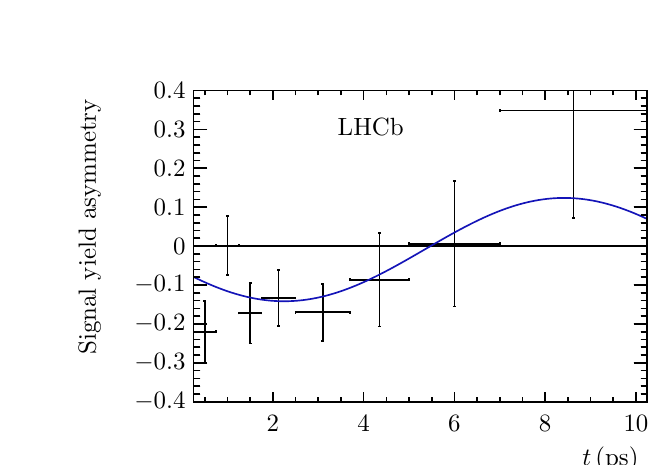
\begin{tikzpicture}[scale=0.38]
\pgfdeclareplotmark{cross} {
\pgfpathmoveto{\pgfpoint{-0.3\pgfplotmarksize}{\pgfplotmarksize}}
\pgfpathlineto{\pgfpoint{+0.3\pgfplotmarksize}{\pgfplotmarksize}}
\pgfpathlineto{\pgfpoint{+0.3\pgfplotmarksize}{0.3\pgfplotmarksize}}
\pgfpathlineto{\pgfpoint{+1\pgfplotmarksize}{0.3\pgfplotmarksize}}
\pgfpathlineto{\pgfpoint{+1\pgfplotmarksize}{-0.3\pgfplotmarksize}}
\pgfpathlineto{\pgfpoint{+0.3\pgfplotmarksize}{-0.3\pgfplotmarksize}}
\pgfpathlineto{\pgfpoint{+0.3\pgfplotmarksize}{-1.\pgfplotmarksize}}
\pgfpathlineto{\pgfpoint{-0.3\pgfplotmarksize}{-1.\pgfplotmarksize}}
\pgfpathlineto{\pgfpoint{-0.3\pgfplotmarksize}{-0.3\pgfplotmarksize}}
\pgfpathlineto{\pgfpoint{-1.\pgfplotmarksize}{-0.3\pgfplotmarksize}}
\pgfpathlineto{\pgfpoint{-1.\pgfplotmarksize}{0.3\pgfplotmarksize}}
\pgfpathlineto{\pgfpoint{-0.3\pgfplotmarksize}{0.3\pgfplotmarksize}}
\pgfpathclose
\pgfusepathqstroke
}
\pgfdeclareplotmark{cross*} {
\pgfpathmoveto{\pgfpoint{-0.3\pgfplotmarksize}{\pgfplotmarksize}}
\pgfpathlineto{\pgfpoint{+0.3\pgfplotmarksize}{\pgfplotmarksize}}
\pgfpathlineto{\pgfpoint{+0.3\pgfplotmarksize}{0.3\pgfplotmarksize}}
\pgfpathlineto{\pgfpoint{+1\pgfplotmarksize}{0.3\pgfplotmarksize}}
\pgfpathlineto{\pgfpoint{+1\pgfplotmarksize}{-0.3\pgfplotmarksize}}
\pgfpathlineto{\pgfpoint{+0.3\pgfplotmarksize}{-0.3\pgfplotmarksize}}
\pgfpathlineto{\pgfpoint{+0.3\pgfplotmarksize}{-1.\pgfplotmarksize}}
\pgfpathlineto{\pgfpoint{-0.3\pgfplotmarksize}{-1.\pgfplotmarksize}}
\pgfpathlineto{\pgfpoint{-0.3\pgfplotmarksize}{-0.3\pgfplotmarksize}}
\pgfpathlineto{\pgfpoint{-1.\pgfplotmarksize}{-0.3\pgfplotmarksize}}
\pgfpathlineto{\pgfpoint{-1.\pgfplotmarksize}{0.3\pgfplotmarksize}}
\pgfpathlineto{\pgfpoint{-0.3\pgfplotmarksize}{0.3\pgfplotmarksize}}
\pgfpathclose
\pgfusepathqfillstroke
}
\pgfdeclareplotmark{newstar} {
\pgfpathmoveto{\pgfqpoint{0pt}{\pgfplotmarksize}}
\pgfpathlineto{\pgfqpointpolar{44}{0.5\pgfplotmarksize}}
\pgfpathlineto{\pgfqpointpolar{18}{\pgfplotmarksize}}
\pgfpathlineto{\pgfqpointpolar{-20}{0.5\pgfplotmarksize}}
\pgfpathlineto{\pgfqpointpolar{-54}{\pgfplotmarksize}}
\pgfpathlineto{\pgfqpointpolar{-90}{0.5\pgfplotmarksize}}
\pgfpathlineto{\pgfqpointpolar{234}{\pgfplotmarksize}}
\pgfpathlineto{\pgfqpointpolar{198}{0.5\pgfplotmarksize}}
\pgfpathlineto{\pgfqpointpolar{162}{\pgfplotmarksize}}
\pgfpathlineto{\pgfqpointpolar{134}{0.5\pgfplotmarksize}}
\pgfpathclose
\pgfusepathqstroke
}
\pgfdeclareplotmark{newstar*} {
\pgfpathmoveto{\pgfqpoint{0pt}{\pgfplotmarksize}}
\pgfpathlineto{\pgfqpointpolar{44}{0.5\pgfplotmarksize}}
\pgfpathlineto{\pgfqpointpolar{18}{\pgfplotmarksize}}
\pgfpathlineto{\pgfqpointpolar{-20}{0.5\pgfplotmarksize}}
\pgfpathlineto{\pgfqpointpolar{-54}{\pgfplotmarksize}}
\pgfpathlineto{\pgfqpointpolar{-90}{0.5\pgfplotmarksize}}
\pgfpathlineto{\pgfqpointpolar{234}{\pgfplotmarksize}}
\pgfpathlineto{\pgfqpointpolar{198}{0.5\pgfplotmarksize}}
\pgfpathlineto{\pgfqpointpolar{162}{\pgfplotmarksize}}
\pgfpathlineto{\pgfqpointpolar{134}{0.5\pgfplotmarksize}}
\pgfpathclose
\pgfusepathqfillstroke
}
\definecolor{c}{rgb}{1,1,1};
\draw [color=c, fill=c] (0.4,0) rectangle (19.6,13.1687);
\draw [color=c, fill=c] (3.472,2.107) rectangle (18.64,12.5103);
\definecolor{c}{rgb}{0,0,0};
\draw [c,line width=0.6] (3.472,2.107) -- (3.472,12.5103) -- (18.64,12.5103) -- (18.64,2.107) -- (3.472,2.107);
\definecolor{c}{rgb}{1,1,1};
\draw [color=c, fill=c] (3.472,2.107) rectangle (18.64,12.5103);
\definecolor{c}{rgb}{0,0,0};
\draw [c,line width=0.6] (3.472,2.107) -- (3.472,12.5103) -- (18.64,12.5103) -- (18.64,2.107) -- (3.472,2.107);
\draw [c,line width=0.6] (3.472,2.107) -- (18.64,2.107);
\draw [anchor= east] (18.64,0.2) node[scale=0.9, color=c, rotate=0]{$t$\,$\mathrm{(ps)}$};
\draw [c,line width=0.6] (6.1264,2.4191) -- (6.1264,2.107);
\draw [c,line width=0.6] (6.8848,2.26305) -- (6.8848,2.107);
\draw [c,line width=0.6] (7.6432,2.26305) -- (7.6432,2.107);
\draw [c,line width=0.6] (8.4016,2.26305) -- (8.4016,2.107);
\draw [c,line width=0.6] (9.16,2.4191) -- (9.16,2.107);
\draw [c,line width=0.6] (9.9184,2.26305) -- (9.9184,2.107);
\draw [c,line width=0.6] (10.6768,2.26305) -- (10.6768,2.107);
\draw [c,line width=0.6] (11.4352,2.26305) -- (11.4352,2.107);
\draw [c,line width=0.6] (12.1936,2.4191) -- (12.1936,2.107);
\draw [c,line width=0.6] (12.952,2.26305) -- (12.952,2.107);
\draw [c,line width=0.6] (13.7104,2.26305) -- (13.7104,2.107);
\draw [c,line width=0.6] (14.4688,2.26305) -- (14.4688,2.107);
\draw [c,line width=0.6] (15.2272,2.4191) -- (15.2272,2.107);
\draw [c,line width=0.6] (15.9856,2.26305) -- (15.9856,2.107);
\draw [c,line width=0.6] (16.744,2.26305) -- (16.744,2.107);
\draw [c,line width=0.6] (17.5024,2.26305) -- (17.5024,2.107);
\draw [c,line width=0.6] (18.2608,2.4191) -- (18.2608,2.107);
\draw [c,line width=0.6] (6.1264,2.4191) -- (6.1264,2.107);
\draw [c,line width=0.6] (5.368,2.26305) -- (5.368,2.107);
\draw [c,line width=0.6] (4.6096,2.26305) -- (4.6096,2.107);
\draw [c,line width=0.6] (3.8512,2.26305) -- (3.8512,2.107);
\draw [c,line width=0.6] (18.2608,2.4191) -- (18.2608,2.107);
\draw [anchor=base] (6.1264,1.1) node[scale=0.9, color=c, rotate=0]{$2$};
\draw [anchor=base] (9.16,1.1) node[scale=0.9, color=c, rotate=0]{$4$};
\draw [anchor=base] (12.1936,1.1) node[scale=0.9, color=c, rotate=0]{$6$};
\draw [anchor=base] (15.2272,1.1) node[scale=0.9, color=c, rotate=0]{$8$};
\draw [anchor=base] (18.2608,1.1) node[scale=0.9, color=c, rotate=0]{$10$};
\draw [c,line width=0.6] (3.472,12.5103) -- (18.64,12.5103);
\draw [c,line width=0.6] (6.1264,12.1982) -- (6.1264,12.5103);
\draw [c,line width=0.6] (6.8848,12.3543) -- (6.8848,12.5103);
\draw [c,line width=0.6] (7.6432,12.3543) -- (7.6432,12.5103);
\draw [c,line width=0.6] (8.4016,12.3543) -- (8.4016,12.5103);
\draw [c,line width=0.6] (9.16,12.1982) -- (9.16,12.5103);
\draw [c,line width=0.6] (9.9184,12.3543) -- (9.9184,12.5103);
\draw [c,line width=0.6] (10.6768,12.3543) -- (10.6768,12.5103);
\draw [c,line width=0.6] (11.4352,12.3543) -- (11.4352,12.5103);
\draw [c,line width=0.6] (12.1936,12.1982) -- (12.1936,12.5103);
\draw [c,line width=0.6] (12.952,12.3543) -- (12.952,12.5103);
\draw [c,line width=0.6] (13.7104,12.3543) -- (13.7104,12.5103);
\draw [c,line width=0.6] (14.4688,12.3543) -- (14.4688,12.5103);
\draw [c,line width=0.6] (15.2272,12.1982) -- (15.2272,12.5103);
\draw [c,line width=0.6] (15.9856,12.3543) -- (15.9856,12.5103);
\draw [c,line width=0.6] (16.744,12.3543) -- (16.744,12.5103);
\draw [c,line width=0.6] (17.5024,12.3543) -- (17.5024,12.5103);
\draw [c,line width=0.6] (18.2608,12.1982) -- (18.2608,12.5103);
\draw [c,line width=0.6] (6.1264,12.1982) -- (6.1264,12.5103);
\draw [c,line width=0.6] (5.368,12.3543) -- (5.368,12.5103);
\draw [c,line width=0.6] (4.6096,12.3543) -- (4.6096,12.5103);
\draw [c,line width=0.6] (3.8512,12.3543) -- (3.8512,12.5103);
\draw [c,line width=0.6] (18.2608,12.1982) -- (18.2608,12.5103);
\draw [c,line width=0.6] (3.472,2.107) -- (3.472,12.5103);
\draw [anchor= east] (0.,12.5103) node[scale=0.9, color=c, rotate=90]{Signal yield asymmetry};
\draw [c,line width=0.6] (3.92704,2.107) -- (3.472,2.107);
\draw [c,line width=0.6] (3.69952,2.36708) -- (3.472,2.36708);
\draw [c,line width=0.6] (3.69952,2.62717) -- (3.472,2.62717);
\draw [c,line width=0.6] (3.69952,2.88725) -- (3.472,2.88725);
\draw [c,line width=0.6] (3.69952,3.14733) -- (3.472,3.14733);
\draw [c,line width=0.6] (3.92704,3.40741) -- (3.472,3.40741);
\draw [c,line width=0.6] (3.69952,3.6675) -- (3.472,3.6675);
\draw [c,line width=0.6] (3.69952,3.92758) -- (3.472,3.92758);
\draw [c,line width=0.6] (3.69952,4.18766) -- (3.472,4.18766);
\draw [c,line width=0.6] (3.69952,4.44775) -- (3.472,4.44775);
\draw [c,line width=0.6] (3.92704,4.70783) -- (3.472,4.70783);
\draw [c,line width=0.6] (3.69952,4.96791) -- (3.472,4.96791);
\draw [c,line width=0.6] (3.69952,5.22799) -- (3.472,5.22799);
\draw [c,line width=0.6] (3.69952,5.48808) -- (3.472,5.48808);
\draw [c,line width=0.6] (3.69952,5.74816) -- (3.472,5.74816);
\draw [c,line width=0.6] (3.92704,6.00824) -- (3.472,6.00824);
\draw [c,line width=0.6] (3.69952,6.26832) -- (3.472,6.26832);
\draw [c,line width=0.6] (3.69952,6.52841) -- (3.472,6.52841);
\draw [c,line width=0.6] (3.69952,6.78849) -- (3.472,6.78849);
\draw [c,line width=0.6] (3.69952,7.04857) -- (3.472,7.04857);
\draw [c,line width=0.6] (3.92704,7.30866) -- (3.472,7.30866);
\draw [c,line width=0.6] (3.69952,7.56874) -- (3.472,7.56874);
\draw [c,line width=0.6] (3.69952,7.82882) -- (3.472,7.82882);
\draw [c,line width=0.6] (3.69952,8.0889) -- (3.472,8.0889);
\draw [c,line width=0.6] (3.69952,8.34899) -- (3.472,8.34899);
\draw [c,line width=0.6] (3.92704,8.60907) -- (3.472,8.60907);
\draw [c,line width=0.6] (3.69952,8.86915) -- (3.472,8.86915);
\draw [c,line width=0.6] (3.69952,9.12924) -- (3.472,9.12924);
\draw [c,line width=0.6] (3.69952,9.38932) -- (3.472,9.38932);
\draw [c,line width=0.6] (3.69952,9.6494) -- (3.472,9.6494);
\draw [c,line width=0.6] (3.92704,9.90948) -- (3.472,9.90948);
\draw [c,line width=0.6] (3.69952,10.1696) -- (3.472,10.1696);
\draw [c,line width=0.6] (3.69952,10.4297) -- (3.472,10.4297);
\draw [c,line width=0.6] (3.69952,10.6897) -- (3.472,10.6897);
\draw [c,line width=0.6] (3.69952,10.9498) -- (3.472,10.9498);
\draw [c,line width=0.6] (3.92704,11.2099) -- (3.472,11.2099);
\draw [c,line width=0.6] (3.69952,11.47) -- (3.472,11.47);
\draw [c,line width=0.6] (3.69952,11.7301) -- (3.472,11.7301);
\draw [c,line width=0.6] (3.69952,11.9901) -- (3.472,11.9901);
\draw [c,line width=0.6] (3.69952,12.2502) -- (3.472,12.2502);
\draw [c,line width=0.6] (3.92704,12.5103) -- (3.472,12.5103);
\draw [anchor= east] (3.5,2.107) node[scale=0.9, color=c, rotate=0]{$-0.4$};
\draw [anchor= east] (3.5,3.40741) node[scale=0.9, color=c, rotate=0]{$-0.3$};
\draw [anchor= east] (3.5,4.70783) node[scale=0.9, color=c, rotate=0]{$-0.2$};
\draw [anchor= east] (3.5,6.00824) node[scale=0.9, color=c, rotate=0]{$-0.1$};
\draw [anchor= east] (3.5,7.30866) node[scale=0.9, color=c, rotate=0]{$0$};
\draw [anchor= east] (3.5,8.60907) node[scale=0.9, color=c, rotate=0]{$0.1$};
\draw [anchor= east] (3.5,9.90948) node[scale=0.9, color=c, rotate=0]{$0.2$};
\draw [anchor= east] (3.5,11.2099) node[scale=0.9, color=c, rotate=0]{$0.3$};
\draw [anchor= east] (3.5,12.5103) node[scale=0.9, color=c, rotate=0]{$0.4$};
\draw [c,line width=0.6] (18.64,2.107) -- (18.64,12.5103);
\draw [c,line width=0.6] (18.185,2.107) -- (18.64,2.107);
\draw [c,line width=0.6] (18.4125,2.36708) -- (18.64,2.36708);
\draw [c,line width=0.6] (18.4125,2.62717) -- (18.64,2.62717);
\draw [c,line width=0.6] (18.4125,2.88725) -- (18.64,2.88725);
\draw [c,line width=0.6] (18.4125,3.14733) -- (18.64,3.14733);
\draw [c,line width=0.6] (18.185,3.40741) -- (18.64,3.40741);
\draw [c,line width=0.6] (18.4125,3.6675) -- (18.64,3.6675);
\draw [c,line width=0.6] (18.4125,3.92758) -- (18.64,3.92758);
\draw [c,line width=0.6] (18.4125,4.18766) -- (18.64,4.18766);
\draw [c,line width=0.6] (18.4125,4.44775) -- (18.64,4.44775);
\draw [c,line width=0.6] (18.185,4.70783) -- (18.64,4.70783);
\draw [c,line width=0.6] (18.4125,4.96791) -- (18.64,4.96791);
\draw [c,line width=0.6] (18.4125,5.22799) -- (18.64,5.22799);
\draw [c,line width=0.6] (18.4125,5.48808) -- (18.64,5.48808);
\draw [c,line width=0.6] (18.4125,5.74816) -- (18.64,5.74816);
\draw [c,line width=0.6] (18.185,6.00824) -- (18.64,6.00824);
\draw [c,line width=0.6] (18.4125,6.26832) -- (18.64,6.26832);
\draw [c,line width=0.6] (18.4125,6.52841) -- (18.64,6.52841);
\draw [c,line width=0.6] (18.4125,6.78849) -- (18.64,6.78849);
\draw [c,line width=0.6] (18.4125,7.04857) -- (18.64,7.04857);
\draw [c,line width=0.6] (18.185,7.30866) -- (18.64,7.30866);
\draw [c,line width=0.6] (18.4125,7.56874) -- (18.64,7.56874);
\draw [c,line width=0.6] (18.4125,7.82882) -- (18.64,7.82882);
\draw [c,line width=0.6] (18.4125,8.0889) -- (18.64,8.0889);
\draw [c,line width=0.6] (18.4125,8.34899) -- (18.64,8.34899);
\draw [c,line width=0.6] (18.185,8.60907) -- (18.64,8.60907);
\draw [c,line width=0.6] (18.4125,8.86915) -- (18.64,8.86915);
\draw [c,line width=0.6] (18.4125,9.12924) -- (18.64,9.12924);
\draw [c,line width=0.6] (18.4125,9.38932) -- (18.64,9.38932);
\draw [c,line width=0.6] (18.4125,9.6494) -- (18.64,9.6494);
\draw [c,line width=0.6] (18.185,9.90948) -- (18.64,9.90948);
\draw [c,line width=0.6] (18.4125,10.1696) -- (18.64,10.1696);
\draw [c,line width=0.6] (18.4125,10.4297) -- (18.64,10.4297);
\draw [c,line width=0.6] (18.4125,10.6897) -- (18.64,10.6897);
\draw [c,line width=0.6] (18.4125,10.9498) -- (18.64,10.9498);
\draw [c,line width=0.6] (18.185,11.2099) -- (18.64,11.2099);
\draw [c,line width=0.6] (18.4125,11.47) -- (18.64,11.47);
\draw [c,line width=0.6] (18.4125,11.7301) -- (18.64,11.7301);
\draw [c,line width=0.6] (18.4125,11.9901) -- (18.64,11.9901);
\draw [c,line width=0.6] (18.4125,12.2502) -- (18.64,12.2502);
\draw [c,line width=0.6] (18.185,12.5103) -- (18.64,12.5103);
\draw [c,line width=0.6] (3.8512,4.44769) -- (3.472,4.44769);
\draw [c,line width=0.6] (3.472,4.40304) -- (3.472,4.49233);
\draw [c,line width=0.6] (3.8512,4.44769) -- (4.2304,4.44769);
\draw [c,line width=0.6] (4.2304,4.40304) -- (4.2304,4.49233);
\draw [c,line width=0.6] (3.8512,4.44769) -- (3.8512,5.47943);
\draw [c,line width=0.6] (3.80656,5.47943) -- (3.89584,5.47943);
\draw [c,line width=0.6] (3.8512,4.44769) -- (3.8512,3.41595);
\draw [c,line width=0.6] (3.80656,3.41595) -- (3.89584,3.41595);
\draw [c,line width=0.6] (4.6096,7.32499) -- (4.2304,7.32499);
\draw [c,line width=0.6] (4.2304,7.28034) -- (4.2304,7.36963);
\draw [c,line width=0.6] (4.6096,7.32499) -- (4.9888,7.32499);
\draw [c,line width=0.6] (4.9888,7.28034) -- (4.9888,7.36963);
\draw [c,line width=0.6] (4.6096,7.32499) -- (4.6096,8.31537);
\draw [c,line width=0.6] (4.56496,8.31537) -- (4.65424,8.31537);
\draw [c,line width=0.6] (4.6096,7.32499) -- (4.6096,6.33461);
\draw [c,line width=0.6] (4.56496,6.33461) -- (4.65424,6.33461);
\draw [c,line width=0.6] (5.368,5.06704) -- (4.9888,5.06704);
\draw [c,line width=0.6] (4.9888,5.02239) -- (4.9888,5.11168);
\draw [c,line width=0.6] (5.368,5.06704) -- (5.7472,5.06704);
\draw [c,line width=0.6] (5.7472,5.02239) -- (5.7472,5.11168);
\draw [c,line width=0.6] (5.368,5.06704) -- (5.368,6.07911);
\draw [c,line width=0.6] (5.32336,6.07911) -- (5.41264,6.07911);
\draw [c,line width=0.6] (5.368,5.06704) -- (5.368,4.05496);
\draw [c,line width=0.6] (5.32336,4.05496) -- (5.41264,4.05496);
\draw [c,line width=0.6] (6.316,5.57743) -- (5.7472,5.57743);
\draw [c,line width=0.6] (5.7472,5.53278) -- (5.7472,5.62207);
\draw [c,line width=0.6] (6.316,5.57743) -- (6.8848,5.57743);
\draw [c,line width=0.6] (6.8848,5.53278) -- (6.8848,5.62207);
\draw [c,line width=0.6] (6.316,5.57743) -- (6.316,6.51804);
\draw [c,line width=0.6] (6.27136,6.51804) -- (6.36064,6.51804);
\draw [c,line width=0.6] (6.316,5.57743) -- (6.316,4.63681);
\draw [c,line width=0.6] (6.27136,4.63681) -- (6.36064,4.63681);
\draw [c,line width=0.6] (7.79488,5.09749) -- (6.8848,5.09749);
\draw [c,line width=0.6] (6.8848,5.05284) -- (6.8848,5.14213);
\draw [c,line width=0.6] (7.79488,5.09749) -- (8.70496,5.09749);
\draw [c,line width=0.6] (8.70496,5.05284) -- (8.70496,5.14213);
\draw [c,line width=0.6] (7.79488,5.09749) -- (7.79488,6.04843);
\draw [c,line width=0.6] (7.75024,6.04843) -- (7.83952,6.04843);
\draw [c,line width=0.6] (7.79488,5.09749) -- (7.79488,4.14654);
\draw [c,line width=0.6] (7.75024,4.14654) -- (7.83952,4.14654);
\draw [c,line width=0.6] (9.69088,6.18148) -- (8.70496,6.18148);
\draw [c,line width=0.6] (8.70496,6.13683) -- (8.70496,6.22612);
\draw [c,line width=0.6] (9.69088,6.18148) -- (10.6768,6.18148);
\draw [c,line width=0.6] (10.6768,6.13683) -- (10.6768,6.22612);
\draw [c,line width=0.6] (9.69088,6.18148) -- (9.69088,7.74299);
\draw [c,line width=0.6] (9.64624,7.74299) -- (9.73552,7.74299);
\draw [c,line width=0.6] (9.69088,6.18148) -- (9.69088,4.61996);
\draw [c,line width=0.6] (9.64624,4.61996) -- (9.73552,4.61996);
\draw [c,line width=0.6] (12.1936,7.38514) -- (10.6768,7.38514);
\draw [c,line width=0.6] (10.6768,7.3405) -- (10.6768,7.42978);
\draw [c,line width=0.6] (12.1936,7.38514) -- (13.7104,7.38514);
\draw [c,line width=0.6] (13.7104,7.3405) -- (13.7104,7.42978);
\draw [c,line width=0.6] (12.1936,7.38514) -- (12.1936,9.48546);
\draw [c,line width=0.6] (12.149,9.48546) -- (12.2382,9.48546);
\draw [c,line width=0.6] (12.1936,7.38514) -- (12.1936,5.28482);
\draw [c,line width=0.6] (12.149,5.28482) -- (12.2382,5.28482);
\draw [c,line width=0.6] (16.1752,11.835) -- (13.7104,11.835);
\draw [c,line width=0.6] (13.7104,11.7904) -- (13.7104,11.8796);
\draw [c,line width=0.6] (16.1752,11.835) -- (18.64,11.835);
\draw [c,line width=0.6] (18.64,11.7904) -- (18.64,11.8796);
\draw [c,line width=0.6] (16.1752,11.835) -- (16.1752,12.5103);
\draw [c,line width=0.6] (16.1306,12.5103) -- (16.2198,12.5103);
\draw [c,line width=0.6] (16.1752,11.835) -- (16.1752,8.24828);
\draw [c,line width=0.6] (16.1306,8.24828) -- (16.2198,8.24828);
\foreach \P in {(3.8512,4.44769),(4.6096,7.32499),(5.368,5.06704),(6.316,5.57743),(7.79488,5.09749),(9.69088,6.18148),(12.1936,7.38514),(16.1752,11.835)}{\draw[mark options={color=c,fill=c},mark size=2.402402pt,mark=] plot coordinates {\P};}

\draw [c,line width=0.6] (3.54784,7.30866) -- (3.69952,7.30866) -- (3.8512,7.30866) -- (4.00288,7.30866) -- (4.15456,7.30866) -- (4.30624,7.30866) -- (4.45792,7.30866) -- (4.6096,7.30866) -- (4.76128,7.30866) -- (4.91296,7.30866) -- (5.06464,7.30866) --
 (5.21632,7.30866) -- (5.368,7.30866) -- (5.51968,7.30866) -- (5.67136,7.30866) -- (5.82304,7.30866) -- (5.97472,7.30866) -- (6.1264,7.30866) -- (6.27808,7.30866) -- (6.42976,7.30866) -- (6.58144,7.30866) -- (6.73312,7.30866) -- (6.8848,7.30866) --
 (7.03648,7.30866) -- (7.18816,7.30866) -- (7.33984,7.30866) -- (7.49152,7.30866) -- (7.6432,7.30866) -- (7.79488,7.30866) -- (7.94656,7.30866) -- (8.09824,7.30866) -- (8.24992,7.30866) -- (8.4016,7.30866) -- (8.55328,7.30866) -- (8.70496,7.30866) --
 (8.85664,7.30866) -- (9.00832,7.30866) -- (9.16,7.30866) -- (9.31168,7.30866) -- (9.46336,7.30866) -- (9.61504,7.30866) -- (9.76672,7.30866) -- (9.9184,7.30866) -- (10.0701,7.30866) -- (10.2218,7.30866) -- (10.3734,7.30866) -- (10.5251,7.30866) --
 (10.6768,7.30866) -- (10.8285,7.30866) -- (10.9802,7.30866);
\draw [c,line width=0.6] (10.9802,7.30866) -- (11.1318,7.30866) -- (11.2835,7.30866) -- (11.4352,7.30866) -- (11.5869,7.30866) -- (11.7386,7.30866) -- (11.8902,7.30866) -- (12.0419,7.30866) -- (12.1936,7.30866) -- (12.3453,7.30866) -- (12.497,7.30866) --
 (12.6486,7.30866) -- (12.8003,7.30866) -- (12.952,7.30866) -- (13.1037,7.30866) -- (13.2554,7.30866) -- (13.407,7.30866) -- (13.5587,7.30866) -- (13.7104,7.30866) -- (13.8621,7.30866) -- (14.0138,7.30866) -- (14.1654,7.30866) -- (14.3171,7.30866) --
 (14.4688,7.30866) -- (14.6205,7.30866) -- (14.7722,7.30866) -- (14.9238,7.30866) -- (15.0755,7.30866) -- (15.2272,7.30866) -- (15.3789,7.30866) -- (15.5306,7.30866) -- (15.6822,7.30866) -- (15.8339,7.30866) -- (15.9856,7.30866) -- (16.1373,7.30866)
 -- (16.289,7.30866) -- (16.4406,7.30866) -- (16.5923,7.30866) -- (16.744,7.30866) -- (16.8957,7.30866) -- (17.0474,7.30866) -- (17.199,7.30866) -- (17.3507,7.30866) -- (17.5024,7.30866) -- (17.6541,7.30866) -- (17.8058,7.30866) -- (17.9574,7.30866)
 -- (18.1091,7.30866) -- (18.2608,7.30866) -- (18.4125,7.30866);
\draw [c] (18.4125,7.30866) -- (18.5642,7.30866);

\definecolor{c}{rgb}{0.08,0.08,0.72};
\draw [c,line width=0.6] (3.472,6.279) -- (3.62368,6.20573) -- (3.77536,6.13503) -- (3.92704,6.06705) -- (4.07872,6.00199) -- (4.2304,5.94001) -- (4.38208,5.88126) -- (4.53376,5.8259) -- (4.68544,5.77406) -- (4.83712,5.72588) -- (4.9888,5.68147) --
 (5.14048,5.64096) -- (5.29216,5.60444) -- (5.44384,5.57201) -- (5.59552,5.54374) -- (5.7472,5.51971) -- (5.89888,5.49999) -- (6.05056,5.48461) -- (6.20224,5.47362) -- (6.35392,5.46704) -- (6.5056,5.4649) -- (6.65728,5.4672) -- (6.80896,5.47393) --
 (6.96064,5.48507) -- (7.11232,5.5006) -- (7.264,5.52048) -- (7.41568,5.54466) -- (7.56736,5.57307) -- (7.71904,5.60565) -- (7.87072,5.64231) -- (8.0224,5.68296) -- (8.17408,5.7275) -- (8.32576,5.77581) -- (8.47744,5.82777) -- (8.62912,5.88326) --
 (8.7808,5.94212) -- (8.93248,6.00421) -- (9.08416,6.06937) -- (9.23584,6.13744) -- (9.38752,6.20825) -- (9.5392,6.2816) -- (9.69088,6.35732) -- (9.84256,6.4352) -- (9.99424,6.51506) -- (10.1459,6.59669) -- (10.2976,6.67987) -- (10.4493,6.7644) --
 (10.601,6.85005) -- (10.7526,6.9366) -- (10.9043,7.02384) -- (11.056,7.11153) -- (11.2077,7.19945) -- (11.3594,7.28737) -- (11.511,7.37506) -- (11.6627,7.4623) -- (11.8144,7.54885) -- (11.9661,7.63449) -- (12.1178,7.71901) -- (12.2694,7.80217) --
 (12.4211,7.88376) -- (12.5728,7.96356) -- (12.7245,8.04138) -- (12.8762,8.11699) -- (13.0278,8.19021) -- (13.1795,8.26083) -- (13.3312,8.32868) -- (13.4829,8.39357) -- (13.6346,8.45534) -- (13.7862,8.51382) -- (13.9379,8.56885) -- (14.0896,8.62029)
 -- (14.2413,8.668) -- (14.393,8.71186) -- (14.5446,8.75175) -- (14.6963,8.78756) -- (14.848,8.8192) -- (14.9997,8.84658) -- (15.1514,8.86963) -- (15.303,8.8883) -- (15.4547,8.90252) -- (15.6064,8.91226) -- (15.7581,8.9175) -- (15.9098,8.91823) --
 (16.0614,8.91443) -- (16.2131,8.90612) -- (16.3648,8.89333) -- (16.5165,8.87608) -- (16.6682,8.85442) -- (16.8198,8.82841) -- (16.9715,8.79813) -- (17.1232,8.76364) -- (17.2749,8.72504) -- (17.4266,8.68244) -- (17.5782,8.63595) -- (17.7299,8.58568)
 -- (17.8816,8.53179) -- (18.0333,8.47439) -- (18.185,8.41366) -- (18.3366,8.34975) -- (18.4883,8.28282) -- (18.64,8.21307);
\definecolor{c}{rgb}{0,0,0};
\draw [c,line width=0.6] (3.472,2.107) -- (18.64,2.107);
\draw [c,line width=0.6] (6.1264,2.4191) -- (6.1264,2.107);
\draw [c,line width=0.6] (6.8848,2.26305) -- (6.8848,2.107);
\draw [c,line width=0.6] (7.6432,2.26305) -- (7.6432,2.107);
\draw [c,line width=0.6] (8.4016,2.26305) -- (8.4016,2.107);
\draw [c,line width=0.6] (9.16,2.4191) -- (9.16,2.107);
\draw [c,line width=0.6] (9.9184,2.26305) -- (9.9184,2.107);
\draw [c,line width=0.6] (10.6768,2.26305) -- (10.6768,2.107);
\draw [c,line width=0.6] (11.4352,2.26305) -- (11.4352,2.107);
\draw [c,line width=0.6] (12.1936,2.4191) -- (12.1936,2.107);
\draw [c,line width=0.6] (12.952,2.26305) -- (12.952,2.107);
\draw [c,line width=0.6] (13.7104,2.26305) -- (13.7104,2.107);
\draw [c,line width=0.6] (14.4688,2.26305) -- (14.4688,2.107);
\draw [c,line width=0.6] (15.2272,2.4191) -- (15.2272,2.107);
\draw [c,line width=0.6] (15.9856,2.26305) -- (15.9856,2.107);
\draw [c,line width=0.6] (16.744,2.26305) -- (16.744,2.107);
\draw [c,line width=0.6] (17.5024,2.26305) -- (17.5024,2.107);
\draw [c,line width=0.6] (18.2608,2.4191) -- (18.2608,2.107);
\draw [c,line width=0.6] (6.1264,2.4191) -- (6.1264,2.107);
\draw [c,line width=0.6] (5.368,2.26305) -- (5.368,2.107);
\draw [c,line width=0.6] (4.6096,2.26305) -- (4.6096,2.107);
\draw [c,line width=0.6] (3.8512,2.26305) -- (3.8512,2.107);
\draw [c,line width=0.6] (18.2608,2.4191) -- (18.2608,2.107);
\draw [c,line width=0.6] (3.472,12.5103) -- (18.64,12.5103);
\draw [c,line width=0.6] (6.1264,12.1982) -- (6.1264,12.5103);
\draw [c,line width=0.6] (6.8848,12.3543) -- (6.8848,12.5103);
\draw [c,line width=0.6] (7.6432,12.3543) -- (7.6432,12.5103);
\draw [c,line width=0.6] (8.4016,12.3543) -- (8.4016,12.5103);
\draw [c,line width=0.6] (9.16,12.1982) -- (9.16,12.5103);
\draw [c,line width=0.6] (9.9184,12.3543) -- (9.9184,12.5103);
\draw [c,line width=0.6] (10.6768,12.3543) -- (10.6768,12.5103);
\draw [c,line width=0.6] (11.4352,12.3543) -- (11.4352,12.5103);
\draw [c,line width=0.6] (12.1936,12.1982) -- (12.1936,12.5103);
\draw [c,line width=0.6] (12.952,12.3543) -- (12.952,12.5103);
\draw [c,line width=0.6] (13.7104,12.3543) -- (13.7104,12.5103);
\draw [c,line width=0.6] (14.4688,12.3543) -- (14.4688,12.5103);
\draw [c,line width=0.6] (15.2272,12.1982) -- (15.2272,12.5103);
\draw [c,line width=0.6] (15.9856,12.3543) -- (15.9856,12.5103);
\draw [c,line width=0.6] (16.744,12.3543) -- (16.744,12.5103);
\draw [c,line width=0.6] (17.5024,12.3543) -- (17.5024,12.5103);
\draw [c,line width=0.6] (18.2608,12.1982) -- (18.2608,12.5103);
\draw [c,line width=0.6] (6.1264,12.1982) -- (6.1264,12.5103);
\draw [c,line width=0.6] (5.368,12.3543) -- (5.368,12.5103);
\draw [c,line width=0.6] (4.6096,12.3543) -- (4.6096,12.5103);
\draw [c,line width=0.6] (3.8512,12.3543) -- (3.8512,12.5103);
\draw [c,line width=0.6] (18.2608,12.1982) -- (18.2608,12.5103);
\draw [c,line width=0.6] (3.472,2.107) -- (3.472,12.5103);
\draw [c,line width=0.6] (3.92704,2.107) -- (3.472,2.107);
\draw [c,line width=0.6] (3.69952,2.36708) -- (3.472,2.36708);
\draw [c,line width=0.6] (3.69952,2.62717) -- (3.472,2.62717);
\draw [c,line width=0.6] (3.69952,2.88725) -- (3.472,2.88725);
\draw [c,line width=0.6] (3.69952,3.14733) -- (3.472,3.14733);
\draw [c,line width=0.6] (3.92704,3.40741) -- (3.472,3.40741);
\draw [c,line width=0.6] (3.69952,3.6675) -- (3.472,3.6675);
\draw [c,line width=0.6] (3.69952,3.92758) -- (3.472,3.92758);
\draw [c,line width=0.6] (3.69952,4.18766) -- (3.472,4.18766);
\draw [c,line width=0.6] (3.69952,4.44775) -- (3.472,4.44775);
\draw [c,line width=0.6] (3.92704,4.70783) -- (3.472,4.70783);
\draw [c,line width=0.6] (3.69952,4.96791) -- (3.472,4.96791);
\draw [c,line width=0.6] (3.69952,5.22799) -- (3.472,5.22799);
\draw [c,line width=0.6] (3.69952,5.48808) -- (3.472,5.48808);
\draw [c,line width=0.6] (3.69952,5.74816) -- (3.472,5.74816);
\draw [c,line width=0.6] (3.92704,6.00824) -- (3.472,6.00824);
\draw [c,line width=0.6] (3.69952,6.26832) -- (3.472,6.26832);
\draw [c,line width=0.6] (3.69952,6.52841) -- (3.472,6.52841);
\draw [c,line width=0.6] (3.69952,6.78849) -- (3.472,6.78849);
\draw [c,line width=0.6] (3.69952,7.04857) -- (3.472,7.04857);
\draw [c,line width=0.6] (3.92704,7.30866) -- (3.472,7.30866);
\draw [c,line width=0.6] (3.69952,7.56874) -- (3.472,7.56874);
\draw [c,line width=0.6] (3.69952,7.82882) -- (3.472,7.82882);
\draw [c,line width=0.6] (3.69952,8.0889) -- (3.472,8.0889);
\draw [c,line width=0.6] (3.69952,8.34899) -- (3.472,8.34899);
\draw [c,line width=0.6] (3.92704,8.60907) -- (3.472,8.60907);
\draw [c,line width=0.6] (3.69952,8.86915) -- (3.472,8.86915);
\draw [c,line width=0.6] (3.69952,9.12924) -- (3.472,9.12924);
\draw [c,line width=0.6] (3.69952,9.38932) -- (3.472,9.38932);
\draw [c,line width=0.6] (3.69952,9.6494) -- (3.472,9.6494);
\draw [c,line width=0.6] (3.92704,9.90948) -- (3.472,9.90948);
\draw [c,line width=0.6] (3.69952,10.1696) -- (3.472,10.1696);
\draw [c,line width=0.6] (3.69952,10.4297) -- (3.472,10.4297);
\draw [c,line width=0.6] (3.69952,10.6897) -- (3.472,10.6897);
\draw [c,line width=0.6] (3.69952,10.9498) -- (3.472,10.9498);
\draw [c,line width=0.6] (3.92704,11.2099) -- (3.472,11.2099);
\draw [c,line width=0.6] (3.69952,11.47) -- (3.472,11.47);
\draw [c,line width=0.6] (3.69952,11.7301) -- (3.472,11.7301);
\draw [c,line width=0.6] (3.69952,11.9901) -- (3.472,11.9901);
\draw [c,line width=0.6] (3.69952,12.2502) -- (3.472,12.2502);
\draw [c,line width=0.6] (3.92704,12.5103) -- (3.472,12.5103);
\draw [c,line width=0.6] (18.64,2.107) -- (18.64,12.5103);
\draw [c,line width=0.6] (18.185,2.107) -- (18.64,2.107);
\draw [c,line width=0.6] (18.4125,2.36708) -- (18.64,2.36708);
\draw [c,line width=0.6] (18.4125,2.62717) -- (18.64,2.62717);
\draw [c,line width=0.6] (18.4125,2.88725) -- (18.64,2.88725);
\draw [c,line width=0.6] (18.4125,3.14733) -- (18.64,3.14733);
\draw [c,line width=0.6] (18.185,3.40741) -- (18.64,3.40741);
\draw [c,line width=0.6] (18.4125,3.6675) -- (18.64,3.6675);
\draw [c,line width=0.6] (18.4125,3.92758) -- (18.64,3.92758);
\draw [c,line width=0.6] (18.4125,4.18766) -- (18.64,4.18766);
\draw [c,line width=0.6] (18.4125,4.44775) -- (18.64,4.44775);
\draw [c,line width=0.6] (18.185,4.70783) -- (18.64,4.70783);
\draw [c,line width=0.6] (18.4125,4.96791) -- (18.64,4.96791);
\draw [c,line width=0.6] (18.4125,5.22799) -- (18.64,5.22799);
\draw [c,line width=0.6] (18.4125,5.48808) -- (18.64,5.48808);
\draw [c,line width=0.6] (18.4125,5.74816) -- (18.64,5.74816);
\draw [c,line width=0.6] (18.185,6.00824) -- (18.64,6.00824);
\draw [c,line width=0.6] (18.4125,6.26832) -- (18.64,6.26832);
\draw [c,line width=0.6] (18.4125,6.52841) -- (18.64,6.52841);
\draw [c,line width=0.6] (18.4125,6.78849) -- (18.64,6.78849);
\draw [c,line width=0.6] (18.4125,7.04857) -- (18.64,7.04857);
\draw [c,line width=0.6] (18.185,7.30866) -- (18.64,7.30866);
\draw [c,line width=0.6] (18.4125,7.56874) -- (18.64,7.56874);
\draw [c,line width=0.6] (18.4125,7.82882) -- (18.64,7.82882);
\draw [c,line width=0.6] (18.4125,8.0889) -- (18.64,8.0889);
\draw [c,line width=0.6] (18.4125,8.34899) -- (18.64,8.34899);
\draw [c,line width=0.6] (18.185,8.60907) -- (18.64,8.60907);
\draw [c,line width=0.6] (18.4125,8.86915) -- (18.64,8.86915);
\draw [c,line width=0.6] (18.4125,9.12924) -- (18.64,9.12924);
\draw [c,line width=0.6] (18.4125,9.38932) -- (18.64,9.38932);
\draw [c,line width=0.6] (18.4125,9.6494) -- (18.64,9.6494);
\draw [c,line width=0.6] (18.185,9.90948) -- (18.64,9.90948);
\draw [c,line width=0.6] (18.4125,10.1696) -- (18.64,10.1696);
\draw [c,line width=0.6] (18.4125,10.4297) -- (18.64,10.4297);
\draw [c,line width=0.6] (18.4125,10.6897) -- (18.64,10.6897);
\draw [c,line width=0.6] (18.4125,10.9498) -- (18.64,10.9498);
\draw [c,line width=0.6] (18.185,11.2099) -- (18.64,11.2099);
\draw [c,line width=0.6] (18.4125,11.47) -- (18.64,11.47);
\draw [c,line width=0.6] (18.4125,11.7301) -- (18.64,11.7301);
\draw [c,line width=0.6] (18.4125,11.9901) -- (18.64,11.9901);
\draw [c,line width=0.6] (18.4125,12.2502) -- (18.64,12.2502);
\draw [c,line width=0.6] (18.185,12.5103) -- (18.64,12.5103);
\draw [anchor=base west, align=left] (8,10) node[scale=0.9, color=c, rotate=0]{LHCb\\\BdToDD};

\end{tikzpicture}
\endpgfgraphicnamed

\beginpgfgraphicnamed{pdf/Asymmetry_B2JPsiKS}
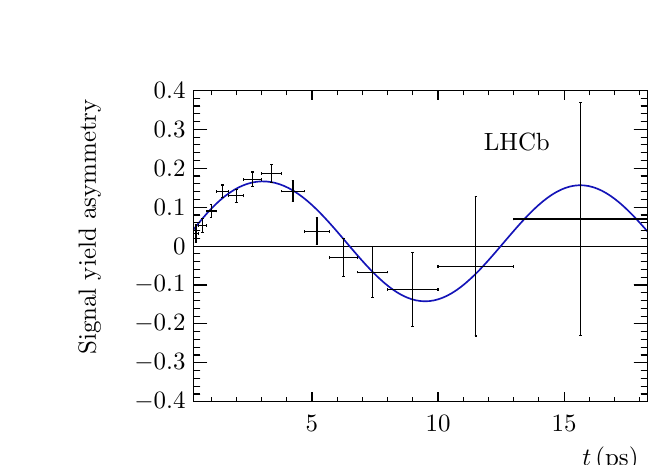
\begin{tikzpicture}[scale=0.38]
\pgfdeclareplotmark{cross} {
\pgfpathmoveto{\pgfpoint{-0.3\pgfplotmarksize}{\pgfplotmarksize}}
\pgfpathlineto{\pgfpoint{+0.3\pgfplotmarksize}{\pgfplotmarksize}}
\pgfpathlineto{\pgfpoint{+0.3\pgfplotmarksize}{0.3\pgfplotmarksize}}
\pgfpathlineto{\pgfpoint{+1\pgfplotmarksize}{0.3\pgfplotmarksize}}
\pgfpathlineto{\pgfpoint{+1\pgfplotmarksize}{-0.3\pgfplotmarksize}}
\pgfpathlineto{\pgfpoint{+0.3\pgfplotmarksize}{-0.3\pgfplotmarksize}}
\pgfpathlineto{\pgfpoint{+0.3\pgfplotmarksize}{-1.\pgfplotmarksize}}
\pgfpathlineto{\pgfpoint{-0.3\pgfplotmarksize}{-1.\pgfplotmarksize}}
\pgfpathlineto{\pgfpoint{-0.3\pgfplotmarksize}{-0.3\pgfplotmarksize}}
\pgfpathlineto{\pgfpoint{-1.\pgfplotmarksize}{-0.3\pgfplotmarksize}}
\pgfpathlineto{\pgfpoint{-1.\pgfplotmarksize}{0.3\pgfplotmarksize}}
\pgfpathlineto{\pgfpoint{-0.3\pgfplotmarksize}{0.3\pgfplotmarksize}}
\pgfpathclose
\pgfusepathqstroke
}
\pgfdeclareplotmark{cross*} {
\pgfpathmoveto{\pgfpoint{-0.3\pgfplotmarksize}{\pgfplotmarksize}}
\pgfpathlineto{\pgfpoint{+0.3\pgfplotmarksize}{\pgfplotmarksize}}
\pgfpathlineto{\pgfpoint{+0.3\pgfplotmarksize}{0.3\pgfplotmarksize}}
\pgfpathlineto{\pgfpoint{+1\pgfplotmarksize}{0.3\pgfplotmarksize}}
\pgfpathlineto{\pgfpoint{+1\pgfplotmarksize}{-0.3\pgfplotmarksize}}
\pgfpathlineto{\pgfpoint{+0.3\pgfplotmarksize}{-0.3\pgfplotmarksize}}
\pgfpathlineto{\pgfpoint{+0.3\pgfplotmarksize}{-1.\pgfplotmarksize}}
\pgfpathlineto{\pgfpoint{-0.3\pgfplotmarksize}{-1.\pgfplotmarksize}}
\pgfpathlineto{\pgfpoint{-0.3\pgfplotmarksize}{-0.3\pgfplotmarksize}}
\pgfpathlineto{\pgfpoint{-1.\pgfplotmarksize}{-0.3\pgfplotmarksize}}
\pgfpathlineto{\pgfpoint{-1.\pgfplotmarksize}{0.3\pgfplotmarksize}}
\pgfpathlineto{\pgfpoint{-0.3\pgfplotmarksize}{0.3\pgfplotmarksize}}
\pgfpathclose
\pgfusepathqfillstroke
}
\pgfdeclareplotmark{newstar} {
\pgfpathmoveto{\pgfqpoint{0pt}{\pgfplotmarksize}}
\pgfpathlineto{\pgfqpointpolar{44}{0.5\pgfplotmarksize}}
\pgfpathlineto{\pgfqpointpolar{18}{\pgfplotmarksize}}
\pgfpathlineto{\pgfqpointpolar{-20}{0.5\pgfplotmarksize}}
\pgfpathlineto{\pgfqpointpolar{-54}{\pgfplotmarksize}}
\pgfpathlineto{\pgfqpointpolar{-90}{0.5\pgfplotmarksize}}
\pgfpathlineto{\pgfqpointpolar{234}{\pgfplotmarksize}}
\pgfpathlineto{\pgfqpointpolar{198}{0.5\pgfplotmarksize}}
\pgfpathlineto{\pgfqpointpolar{162}{\pgfplotmarksize}}
\pgfpathlineto{\pgfqpointpolar{134}{0.5\pgfplotmarksize}}
\pgfpathclose
\pgfusepathqstroke
}
\pgfdeclareplotmark{newstar*} {
\pgfpathmoveto{\pgfqpoint{0pt}{\pgfplotmarksize}}
\pgfpathlineto{\pgfqpointpolar{44}{0.5\pgfplotmarksize}}
\pgfpathlineto{\pgfqpointpolar{18}{\pgfplotmarksize}}
\pgfpathlineto{\pgfqpointpolar{-20}{0.5\pgfplotmarksize}}
\pgfpathlineto{\pgfqpointpolar{-54}{\pgfplotmarksize}}
\pgfpathlineto{\pgfqpointpolar{-90}{0.5\pgfplotmarksize}}
\pgfpathlineto{\pgfqpointpolar{234}{\pgfplotmarksize}}
\pgfpathlineto{\pgfqpointpolar{198}{0.5\pgfplotmarksize}}
\pgfpathlineto{\pgfqpointpolar{162}{\pgfplotmarksize}}
\pgfpathlineto{\pgfqpointpolar{134}{0.5\pgfplotmarksize}}
\pgfpathclose
\pgfusepathqfillstroke
}

% \definecolor{csig}{RGB}{24,90,169}
\definecolor{csig}{rgb}{0.08,0.08,0.72};

\definecolor{c}{rgb}{1,1,1};
\draw [color=c, fill=c] (0.4,0) rectangle (19.6,13.1687);
\draw [color=c, fill=c] (3.472,2.107) rectangle (18.64,12.5103);
\definecolor{c}{rgb}{0,0,0};
\draw [c] (3.472,2.107) -- (3.472,12.5103) -- (18.64,12.5103) -- (18.64,2.107) -- (3.472,2.107);
\definecolor{c}{rgb}{1,1,1};
\draw [color=c, fill=c] (3.472,2.107) rectangle (18.64,12.5103);
\definecolor{c}{rgb}{0,0,0};
\draw [c] (3.472,2.107) -- (3.472,12.5103) -- (18.64,12.5103) -- (18.64,2.107) -- (3.472,2.107);
\draw [c] (3.472,2.107) -- (18.64,2.107);
\draw [anchor= east] (18.64,0.2) node[scale=0.9, rotate=0]{$t$\,$\mathrm{(ps)}$};
\draw [c] (7.43253,2.4191) -- (7.43253,2.107);
\draw [c] (8.2752,2.26305) -- (8.2752,2.107);
\draw [c] (9.11787,2.26305) -- (9.11787,2.107);
\draw [c] (9.96053,2.26305) -- (9.96053,2.107);
\draw [c] (10.8032,2.26305) -- (10.8032,2.107);
\draw [c] (11.6459,2.4191) -- (11.6459,2.107);
\draw [c] (12.4885,2.26305) -- (12.4885,2.107);
\draw [c] (13.3312,2.26305) -- (13.3312,2.107);
\draw [c] (14.1739,2.26305) -- (14.1739,2.107);
\draw [c] (15.0165,2.26305) -- (15.0165,2.107);
\draw [c] (15.8592,2.4191) -- (15.8592,2.107);
\draw [c] (7.43253,2.4191) -- (7.43253,2.107);
\draw [c] (6.58987,2.26305) -- (6.58987,2.107);
\draw [c] (5.7472,2.26305) -- (5.7472,2.107);
\draw [c] (4.90453,2.26305) -- (4.90453,2.107);
\draw [c] (4.06187,2.26305) -- (4.06187,2.107);
\draw [c] (15.8592,2.4191) -- (15.8592,2.107);
\draw [c] (16.7019,2.26305) -- (16.7019,2.107);
\draw [c] (17.5445,2.26305) -- (17.5445,2.107);
\draw [c] (18.3872,2.26305) -- (18.3872,2.107);
\draw [anchor=base] (7.43253,1.1) node[scale=0.9, rotate=0]{$5$};
\draw [anchor=base] (11.6459,1.1) node[scale=0.9, rotate=0]{$10$};
\draw [anchor=base] (15.8592,1.1) node[scale=0.9, rotate=0]{$15$};
\draw [c] (3.472,12.5103) -- (18.64,12.5103);
\draw [c] (7.43253,12.1982) -- (7.43253,12.5103);
\draw [c] (8.2752,12.3543) -- (8.2752,12.5103);
\draw [c] (9.11787,12.3543) -- (9.11787,12.5103);
\draw [c] (9.96053,12.3543) -- (9.96053,12.5103);
\draw [c] (10.8032,12.3543) -- (10.8032,12.5103);
\draw [c] (11.6459,12.1982) -- (11.6459,12.5103);
\draw [c] (12.4885,12.3543) -- (12.4885,12.5103);
\draw [c] (13.3312,12.3543) -- (13.3312,12.5103);
\draw [c] (14.1739,12.3543) -- (14.1739,12.5103);
\draw [c] (15.0165,12.3543) -- (15.0165,12.5103);
\draw [c] (15.8592,12.1982) -- (15.8592,12.5103);
\draw [c] (7.43253,12.1982) -- (7.43253,12.5103);
\draw [c] (6.58987,12.3543) -- (6.58987,12.5103);
\draw [c] (5.7472,12.3543) -- (5.7472,12.5103);
\draw [c] (4.90453,12.3543) -- (4.90453,12.5103);
\draw [c] (4.06187,12.3543) -- (4.06187,12.5103);
\draw [c] (15.8592,12.1982) -- (15.8592,12.5103);
\draw [c] (16.7019,12.3543) -- (16.7019,12.5103);
\draw [c] (17.5445,12.3543) -- (17.5445,12.5103);
\draw [c] (18.3872,12.3543) -- (18.3872,12.5103);
\draw [c] (3.472,2.107) -- (3.472,12.5103);
\draw [anchor= east] (0.,12.5103) node[scale=0.9, rotate=90]{Signal yield asymmetry};
\draw [c] (3.92704,2.107) -- (3.472,2.107);
\draw [c] (3.69952,2.36708) -- (3.472,2.36708);
\draw [c] (3.69952,2.62717) -- (3.472,2.62717);
\draw [c] (3.69952,2.88725) -- (3.472,2.88725);
\draw [c] (3.69952,3.14733) -- (3.472,3.14733);
\draw [c] (3.92704,3.40741) -- (3.472,3.40741);
\draw [c] (3.69952,3.6675) -- (3.472,3.6675);
\draw [c] (3.69952,3.92758) -- (3.472,3.92758);
\draw [c] (3.69952,4.18766) -- (3.472,4.18766);
\draw [c] (3.69952,4.44775) -- (3.472,4.44775);
\draw [c] (3.92704,4.70783) -- (3.472,4.70783);
\draw [c] (3.69952,4.96791) -- (3.472,4.96791);
\draw [c] (3.69952,5.22799) -- (3.472,5.22799);
\draw [c] (3.69952,5.48808) -- (3.472,5.48808);
\draw [c] (3.69952,5.74816) -- (3.472,5.74816);
\draw [c] (3.92704,6.00824) -- (3.472,6.00824);
\draw [c] (3.69952,6.26832) -- (3.472,6.26832);
\draw [c] (3.69952,6.52841) -- (3.472,6.52841);
\draw [c] (3.69952,6.78849) -- (3.472,6.78849);
\draw [c] (3.69952,7.04857) -- (3.472,7.04857);
\draw [c] (3.92704,7.30866) -- (3.472,7.30866);
\draw [c] (3.69952,7.56874) -- (3.472,7.56874);
\draw [c] (3.69952,7.82882) -- (3.472,7.82882);
\draw [c] (3.69952,8.0889) -- (3.472,8.0889);
\draw [c] (3.69952,8.34899) -- (3.472,8.34899);
\draw [c] (3.92704,8.60907) -- (3.472,8.60907);
\draw [c] (3.69952,8.86915) -- (3.472,8.86915);
\draw [c] (3.69952,9.12924) -- (3.472,9.12924);
\draw [c] (3.69952,9.38932) -- (3.472,9.38932);
\draw [c] (3.69952,9.6494) -- (3.472,9.6494);
\draw [c] (3.92704,9.90948) -- (3.472,9.90948);
\draw [c] (3.69952,10.1696) -- (3.472,10.1696);
\draw [c] (3.69952,10.4297) -- (3.472,10.4297);
\draw [c] (3.69952,10.6897) -- (3.472,10.6897);
\draw [c] (3.69952,10.9498) -- (3.472,10.9498);
\draw [c] (3.92704,11.2099) -- (3.472,11.2099);
\draw [c] (3.69952,11.47) -- (3.472,11.47);
\draw [c] (3.69952,11.7301) -- (3.472,11.7301);
\draw [c] (3.69952,11.9901) -- (3.472,11.9901);
\draw [c] (3.69952,12.2502) -- (3.472,12.2502);
\draw [c] (3.92704,12.5103) -- (3.472,12.5103);
\draw [anchor= east] (3.5,2.107)   node[scale=0.9, rotate=0]{$-0.4$};
\draw [anchor= east] (3.5,3.40741) node[scale=0.9, rotate=0]{$-0.3$};
\draw [anchor= east] (3.5,4.70783) node[scale=0.9, rotate=0]{$-0.2$};
\draw [anchor= east] (3.5,6.00824) node[scale=0.9, rotate=0]{$-0.1$};
\draw [anchor= east] (3.5,7.30866) node[scale=0.9, rotate=0]{$0$};
\draw [anchor= east] (3.5,8.60907) node[scale=0.9, rotate=0]{$0.1$};
\draw [anchor= east] (3.5,9.90948) node[scale=0.9, rotate=0]{$0.2$};
\draw [anchor= east] (3.5,11.2099) node[scale=0.9, rotate=0]{$0.3$};
\draw [anchor= east] (3.5,12.5103) node[scale=0.9, rotate=0]{$0.4$};
\draw [c] (18.64,2.107) -- (18.64,12.5103);
\draw [c] (18.185,2.107) -- (18.64,2.107);
\draw [c] (18.4125,2.36708) -- (18.64,2.36708);
\draw [c] (18.4125,2.62717) -- (18.64,2.62717);
\draw [c] (18.4125,2.88725) -- (18.64,2.88725);
\draw [c] (18.4125,3.14733) -- (18.64,3.14733);
\draw [c] (18.185,3.40741) -- (18.64,3.40741);
\draw [c] (18.4125,3.6675) -- (18.64,3.6675);
\draw [c] (18.4125,3.92758) -- (18.64,3.92758);
\draw [c] (18.4125,4.18766) -- (18.64,4.18766);
\draw [c] (18.4125,4.44775) -- (18.64,4.44775);
\draw [c] (18.185,4.70783) -- (18.64,4.70783);
\draw [c] (18.4125,4.96791) -- (18.64,4.96791);
\draw [c] (18.4125,5.22799) -- (18.64,5.22799);
\draw [c] (18.4125,5.48808) -- (18.64,5.48808);
\draw [c] (18.4125,5.74816) -- (18.64,5.74816);
\draw [c] (18.185,6.00824) -- (18.64,6.00824);
\draw [c] (18.4125,6.26832) -- (18.64,6.26832);
\draw [c] (18.4125,6.52841) -- (18.64,6.52841);
\draw [c] (18.4125,6.78849) -- (18.64,6.78849);
\draw [c] (18.4125,7.04857) -- (18.64,7.04857);
\draw [c] (18.185,7.30866) -- (18.64,7.30866);
\draw [c] (18.4125,7.56874) -- (18.64,7.56874);
\draw [c] (18.4125,7.82882) -- (18.64,7.82882);
\draw [c] (18.4125,8.0889) -- (18.64,8.0889);
\draw [c] (18.4125,8.34899) -- (18.64,8.34899);
\draw [c] (18.185,8.60907) -- (18.64,8.60907);
\draw [c] (18.4125,8.86915) -- (18.64,8.86915);
\draw [c] (18.4125,9.12924) -- (18.64,9.12924);
\draw [c] (18.4125,9.38932) -- (18.64,9.38932);
\draw [c] (18.4125,9.6494) -- (18.64,9.6494);
\draw [c] (18.185,9.90948) -- (18.64,9.90948);
\draw [c] (18.4125,10.1696) -- (18.64,10.1696);
\draw [c] (18.4125,10.4297) -- (18.64,10.4297);
\draw [c] (18.4125,10.6897) -- (18.64,10.6897);
\draw [c] (18.4125,10.9498) -- (18.64,10.9498);
\draw [c] (18.185,11.2099) -- (18.64,11.2099);
\draw [c] (18.4125,11.47) -- (18.64,11.47);
\draw [c] (18.4125,11.7301) -- (18.64,11.7301);
\draw [c] (18.4125,11.9901) -- (18.64,11.9901);
\draw [c] (18.4125,12.2502) -- (18.64,12.2502);
\draw [c] (18.185,12.5103) -- (18.64,12.5103);
\draw [c] (3.55627,7.72485) -- (3.472,7.72485);
\draw [c] (3.472,7.68021) -- (3.472,7.7695);
\draw [c] (3.55627,7.72485) -- (3.64053,7.72485);
\draw [c] (3.64053,7.68021) -- (3.64053,7.7695);
\draw [c] (3.55627,7.72485) -- (3.55627,8.0317);
\draw [c] (3.51162,8.0317) -- (3.60091,8.0317);
\draw [c] (3.55627,7.72485) -- (3.55627,7.41801);
\draw [c] (3.51162,7.41801) -- (3.60091,7.41801);
\draw [c] (3.76693,7.99845) -- (3.64053,7.99845);
\draw [c] (3.64053,7.9538) -- (3.64053,8.04309);
\draw [c] (3.76693,7.99845) -- (3.89333,7.99845);
\draw [c] (3.89333,7.9538) -- (3.89333,8.04309);
\draw [c] (3.76693,7.99845) -- (3.76693,8.23983);
\draw [c] (3.72229,8.23983) -- (3.81158,8.23983);
\draw [c] (3.76693,7.99845) -- (3.76693,7.75706);
\draw [c] (3.72229,7.75706) -- (3.81158,7.75706);
\draw [c] (4.06187,8.48292) -- (3.89333,8.48292);
\draw [c] (3.89333,8.43828) -- (3.89333,8.52756);
\draw [c] (4.06187,8.48292) -- (4.2304,8.48292);
\draw [c] (4.2304,8.43828) -- (4.2304,8.52756);
\draw [c] (4.06187,8.48292) -- (4.06187,8.69191);
\draw [c] (4.01722,8.69191) -- (4.10651,8.69191);
\draw [c] (4.06187,8.48292) -- (4.06187,8.27393);
\draw [c] (4.01722,8.27393) -- (4.10651,8.27393);
\draw [c] (4.44107,9.13937) -- (4.2304,9.13937);
\draw [c] (4.2304,9.09473) -- (4.2304,9.18401);
\draw [c] (4.44107,9.13937) -- (4.65173,9.13937);
\draw [c] (4.65173,9.09473) -- (4.65173,9.18401);
\draw [c] (4.44107,9.13937) -- (4.44107,9.34921);
\draw [c] (4.39642,9.34921) -- (4.48571,9.34921);
\draw [c] (4.44107,9.13937) -- (4.44107,8.92953);
\draw [c] (4.39642,8.92953) -- (4.48571,8.92953);
\draw [c] (4.90453,8.99129) -- (4.65173,8.99129);
\draw [c] (4.65173,8.94665) -- (4.65173,9.03594);
\draw [c] (4.90453,8.99129) -- (5.15733,8.99129);
\draw [c] (5.15733,8.94665) -- (5.15733,9.03594);
\draw [c] (4.90453,8.99129) -- (4.90453,9.20979);
\draw [c] (4.85989,9.20979) -- (4.94918,9.20979);
\draw [c] (4.90453,8.99129) -- (4.90453,8.7728);
\draw [c] (4.85989,8.7728) -- (4.94918,8.7728);
\draw [c] (5.45227,9.53821) -- (5.15733,9.53821);
\draw [c] (5.15733,9.49356) -- (5.15733,9.58285);
\draw [c] (5.45227,9.53821) -- (5.7472,9.53821);
\draw [c] (5.7472,9.49356) -- (5.7472,9.58285);
\draw [c] (5.45227,9.53821) -- (5.45227,9.78334);
\draw [c] (5.40762,9.78334) -- (5.49691,9.78334);
\draw [c] (5.45227,9.53821) -- (5.45227,9.29307);
\draw [c] (5.40762,9.29307) -- (5.49691,9.29307);
\draw [c] (6.08427,9.73341) -- (5.7472,9.73341);
\draw [c] (5.7472,9.68876) -- (5.7472,9.77805);
\draw [c] (6.08427,9.73341) -- (6.42133,9.73341);
\draw [c] (6.42133,9.68876) -- (6.42133,9.77805);
\draw [c] (6.08427,9.73341) -- (6.08427,10.0244);
\draw [c] (6.03962,10.0244) -- (6.12891,10.0244);
\draw [c] (6.08427,9.73341) -- (6.08427,9.44242);
\draw [c] (6.03962,9.44242) -- (6.12891,9.44242);
\draw [c] (6.80053,9.14497) -- (6.42133,9.14497);
\draw [c] (6.42133,9.10033) -- (6.42133,9.18962);
\draw [c] (6.80053,9.14497) -- (7.17973,9.14497);
\draw [c] (7.17973,9.10033) -- (7.17973,9.18962);
\draw [c] (6.80053,9.14497) -- (6.80053,9.49261);
\draw [c] (6.75589,9.49261) -- (6.84518,9.49261);
\draw [c] (6.80053,9.14497) -- (6.80053,8.79734);
\draw [c] (6.75589,8.79734) -- (6.84518,8.79734);
\draw [c] (7.60107,7.8052) -- (7.17973,7.8052);
\draw [c] (7.17973,7.76056) -- (7.17973,7.84985);
\draw [c] (7.60107,7.8052) -- (8.0224,7.8052);
\draw [c] (8.0224,7.76056) -- (8.0224,7.84985);
\draw [c] (7.60107,7.8052) -- (7.60107,8.25309);
\draw [c] (7.55642,8.25309) -- (7.64571,8.25309);
\draw [c] (7.60107,7.8052) -- (7.60107,7.35732);
\draw [c] (7.55642,7.35732) -- (7.64571,7.35732);
\draw [c] (8.48587,6.91766) -- (8.0224,6.91766);
\draw [c] (8.0224,6.87302) -- (8.0224,6.96231);
\draw [c] (8.48587,6.91766) -- (8.94933,6.91766);
\draw [c] (8.94933,6.87302) -- (8.94933,6.96231);
\draw [c] (8.48587,6.91766) -- (8.48587,7.55158);
\draw [c] (8.44122,7.55158) -- (8.53051,7.55158);
\draw [c] (8.48587,6.91766) -- (8.48587,6.28375);
\draw [c] (8.44122,6.28375) -- (8.53051,6.28375);
\draw [c] (9.45493,6.43803) -- (8.94933,6.43803);
\draw [c] (8.94933,6.39339) -- (8.94933,6.48268);
\draw [c] (9.45493,6.43803) -- (9.96053,6.43803);
\draw [c] (9.96053,6.39339) -- (9.96053,6.48268);
\draw [c] (9.45493,6.43803) -- (9.45493,7.29226);
\draw [c] (9.41029,7.29226) -- (9.49958,7.29226);
\draw [c] (9.45493,6.43803) -- (9.45493,5.58381);
\draw [c] (9.41029,5.58381) -- (9.49958,5.58381);
\draw [c] (10.8032,5.85731) -- (9.96053,5.85731);
\draw [c] (9.96053,5.81267) -- (9.96053,5.90196);
\draw [c] (10.8032,5.85731) -- (11.6459,5.85731);
\draw [c] (11.6459,5.81267) -- (11.6459,5.90196);
\draw [c] (10.8032,5.85731) -- (10.8032,7.08927);
\draw [c] (10.7586,7.08927) -- (10.8478,7.08927);
\draw [c] (10.8032,5.85731) -- (10.8032,4.62536);
\draw [c] (10.7586,4.62536) -- (10.8478,4.62536);
\draw [c] (12.9099,6.6293) -- (11.6459,6.6293);
\draw [c] (11.6459,6.58465) -- (11.6459,6.67394);
\draw [c] (12.9099,6.6293) -- (14.1739,6.6293);
\draw [c] (14.1739,6.58465) -- (14.1739,6.67394);
\draw [c] (12.9099,6.6293) -- (12.9099,8.95393);
\draw [c] (12.8652,8.95393) -- (12.9545,8.95393);
\draw [c] (12.9099,6.6293) -- (12.9099,4.30466);
\draw [c] (12.8652,4.30466) -- (12.9545,4.30466);
\draw [c] (16.4069,8.21394) -- (14.1739,8.21394);
\draw [c] (14.1739,8.16929) -- (14.1739,8.25858);
\draw [c] (16.4069,8.21394) -- (18.64,8.21394);
\draw [c] (18.64,8.16929) -- (18.64,8.25858);
\draw [c] (16.4069,8.21394) -- (16.4069,12.0975);
\draw [c] (16.3623,12.0975) -- (16.4516,12.0975);
\draw [c] (16.4069,8.21394) -- (16.4069,4.33041);
\draw [c] (16.3623,4.33041) -- (16.4516,4.33041);
\foreach \P in
 {(3.55627,7.72485),(3.76693,7.99845),(4.06187,8.48292),(4.44107,9.13937),(4.90453,8.99129),(5.45227,9.53821),(6.08427,9.73341),(6.80053,9.14497),(7.60107,7.8052),(8.48587,6.91766),(9.45493,6.43803),(10.8032,5.85731),(12.9099,6.6293),(16.4069,8.21394
)}{\draw[mark options={color=c,fill=c},mark size=2.402402pt,mark=] plot coordinates {\P};}
\draw [c] (3.54784,7.30866) -- (3.69952,7.30866) -- (3.8512,7.30866) -- (4.00288,7.30866) -- (4.15456,7.30866) -- (4.30624,7.30866) -- (4.45792,7.30866) -- (4.6096,7.30866) -- (4.76128,7.30866) -- (4.91296,7.30866) -- (5.06464,7.30866) --
 (5.21632,7.30866) -- (5.368,7.30866) -- (5.51968,7.30866) -- (5.67136,7.30866) -- (5.82304,7.30866) -- (5.97472,7.30866) -- (6.1264,7.30866) -- (6.27808,7.30866) -- (6.42976,7.30866) -- (6.58144,7.30866) -- (6.73312,7.30866) -- (6.8848,7.30866) --
 (7.03648,7.30866) -- (7.18816,7.30866) -- (7.33984,7.30866) -- (7.49152,7.30866) -- (7.6432,7.30866) -- (7.79488,7.30866) -- (7.94656,7.30866) -- (8.09824,7.30866) -- (8.24992,7.30866) -- (8.4016,7.30866) -- (8.55328,7.30866) -- (8.70496,7.30866) --
 (8.85664,7.30866) -- (9.00832,7.30866) -- (9.16,7.30866) -- (9.31168,7.30866) -- (9.46336,7.30866) -- (9.61504,7.30866) -- (9.76672,7.30866) -- (9.9184,7.30866) -- (10.0701,7.30866) -- (10.2218,7.30866) -- (10.3734,7.30866) -- (10.5251,7.30866) --
 (10.6768,7.30866) -- (10.8285,7.30866) -- (10.9802,7.30866);
\draw [c] (10.9802,7.30866) -- (11.1318,7.30866) -- (11.2835,7.30866) -- (11.4352,7.30866) -- (11.5869,7.30866) -- (11.7386,7.30866) -- (11.8902,7.30866) -- (12.0419,7.30866) -- (12.1936,7.30866) -- (12.3453,7.30866) -- (12.497,7.30866) --
 (12.6486,7.30866) -- (12.8003,7.30866) -- (12.952,7.30866) -- (13.1037,7.30866) -- (13.2554,7.30866) -- (13.407,7.30866) -- (13.5587,7.30866) -- (13.7104,7.30866) -- (13.8621,7.30866) -- (14.0138,7.30866) -- (14.1654,7.30866) -- (14.3171,7.30866) --
 (14.4688,7.30866) -- (14.6205,7.30866) -- (14.7722,7.30866) -- (14.9238,7.30866) -- (15.0755,7.30866) -- (15.2272,7.30866) -- (15.3789,7.30866) -- (15.5306,7.30866) -- (15.6822,7.30866) -- (15.8339,7.30866) -- (15.9856,7.30866) -- (16.1373,7.30866)
 -- (16.289,7.30866) -- (16.4406,7.30866) -- (16.5923,7.30866) -- (16.744,7.30866) -- (16.8957,7.30866) -- (17.0474,7.30866) -- (17.199,7.30866) -- (17.3507,7.30866) -- (17.5024,7.30866) -- (17.6541,7.30866) -- (17.8058,7.30866) -- (17.9574,7.30866)
 -- (18.1091,7.30866) -- (18.2608,7.30866) -- (18.4125,7.30866);
\draw [c] (18.4125,7.30866) -- (18.5642,7.30866);
\definecolor{c}{rgb}{0.08,0.08,0.72};
\draw [csig,line width=0.6] (3.472,7.85697) -- (3.62368,8.04849) -- (3.77536,8.23217) -- (3.92704,8.40628) -- (4.07872,8.56942) -- (4.2304,8.7205) -- (4.38208,8.85867) -- (4.53376,8.98333) -- (4.68544,9.09406) -- (4.83712,9.19063) -- (4.9888,9.27292) --
 (5.14048,9.34092) -- (5.29216,9.39464) -- (5.44384,9.43413) -- (5.59552,9.45945) -- (5.7472,9.47063) -- (5.89888,9.46775) -- (6.05056,9.45082) -- (6.20224,9.41993) -- (6.35392,9.37517) -- (6.5056,9.31669) -- (6.65728,9.24471) -- (6.80896,9.15955) --
 (6.96064,9.0616) -- (7.11232,8.95142) -- (7.264,8.82963) -- (7.41568,8.69702) -- (7.56736,8.5545) -- (7.71904,8.40307) -- (7.87072,8.24387) -- (8.0224,8.07811) -- (8.17408,7.90709) -- (8.32576,7.7322) -- (8.47744,7.55484) -- (8.62912,7.37646) --
 (8.7808,7.19854) -- (8.93248,7.02254) -- (9.08416,6.84992) -- (9.23584,6.68209) -- (9.38752,6.52045) -- (9.5392,6.36632) -- (9.69088,6.22097) -- (9.84256,6.08558) -- (9.99424,5.96125) -- (10.1459,5.84899) -- (10.2976,5.74972) -- (10.4493,5.66422) --
 (10.601,5.59319) -- (10.7526,5.53721) -- (10.9043,5.49671) -- (11.056,5.47202) -- (11.2077,5.46333) -- (11.3594,5.47072) -- (11.511,5.49412) -- (11.6627,5.53336) -- (11.8144,5.58809) -- (11.9661,5.65791) -- (12.1178,5.74223) -- (12.2694,5.84038) --
 (12.4211,5.95157) -- (12.5728,6.0749) -- (12.7245,6.20937) -- (12.8762,6.35387) -- (13.0278,6.50722) -- (13.1795,6.66818) -- (13.3312,6.8354) -- (13.4829,7.00751) -- (13.6346,7.18307) -- (13.7862,7.36061) -- (13.9379,7.53864) -- (14.0896,7.71567) --
 (14.2413,7.89018) -- (14.393,8.06071) -- (14.5446,8.22577) -- (14.6963,8.38396) -- (14.848,8.53392) -- (14.9997,8.67434) -- (15.1514,8.804) -- (15.303,8.92178) -- (15.4547,9.02663) -- (15.6064,9.11765) -- (15.7581,9.19404) -- (15.9098,9.2551) --
 (16.0614,9.30032) -- (16.2131,9.32929) -- (16.3648,9.34175) -- (16.5165,9.3376) -- (16.6682,9.31687) -- (16.8198,9.27976) -- (16.9715,9.22657) -- (17.1232,9.15779) -- (17.2749,9.07405) -- (17.4266,8.97603) -- (17.5782,8.86465) -- (17.7299,8.74087)
 -- (17.8816,8.60576) -- (18.0333,8.46051) -- (18.185,8.30638) -- (18.3366,8.14469) -- (18.4883,7.97686) -- (18.64,7.8043);
\definecolor{c}{rgb}{0,0,0};
\draw [c] (3.55627,7.72485) -- (3.472,7.72485);
\draw [c] (3.472,7.68021) -- (3.472,7.7695);
\draw [c] (3.55627,7.72485) -- (3.64053,7.72485);
\draw [c] (3.64053,7.68021) -- (3.64053,7.7695);
\draw [c] (3.55627,7.72485) -- (3.55627,8.0317);
\draw [c] (3.51162,8.0317) -- (3.60091,8.0317);
\draw [c] (3.55627,7.72485) -- (3.55627,7.41801);
\draw [c] (3.51162,7.41801) -- (3.60091,7.41801);
\draw [c] (3.76693,7.99845) -- (3.64053,7.99845);
\draw [c] (3.64053,7.9538) -- (3.64053,8.04309);
\draw [c] (3.76693,7.99845) -- (3.89333,7.99845);
\draw [c] (3.89333,7.9538) -- (3.89333,8.04309);
\draw [c] (3.76693,7.99845) -- (3.76693,8.23983);
\draw [c] (3.72229,8.23983) -- (3.81158,8.23983);
\draw [c] (3.76693,7.99845) -- (3.76693,7.75706);
\draw [c] (3.72229,7.75706) -- (3.81158,7.75706);
\draw [c] (4.06187,8.48292) -- (3.89333,8.48292);
\draw [c] (3.89333,8.43828) -- (3.89333,8.52756);
\draw [c] (4.06187,8.48292) -- (4.2304,8.48292);
\draw [c] (4.2304,8.43828) -- (4.2304,8.52756);
\draw [c] (4.06187,8.48292) -- (4.06187,8.69191);
\draw [c] (4.01722,8.69191) -- (4.10651,8.69191);
\draw [c] (4.06187,8.48292) -- (4.06187,8.27393);
\draw [c] (4.01722,8.27393) -- (4.10651,8.27393);
\draw [c] (4.44107,9.13937) -- (4.2304,9.13937);
\draw [c] (4.2304,9.09473) -- (4.2304,9.18401);
\draw [c] (4.44107,9.13937) -- (4.65173,9.13937);
\draw [c] (4.65173,9.09473) -- (4.65173,9.18401);
\draw [c] (4.44107,9.13937) -- (4.44107,9.34921);
\draw [c] (4.39642,9.34921) -- (4.48571,9.34921);
\draw [c] (4.44107,9.13937) -- (4.44107,8.92953);
\draw [c] (4.39642,8.92953) -- (4.48571,8.92953);
\draw [c] (4.90453,8.99129) -- (4.65173,8.99129);
\draw [c] (4.65173,8.94665) -- (4.65173,9.03594);
\draw [c] (4.90453,8.99129) -- (5.15733,8.99129);
\draw [c] (5.15733,8.94665) -- (5.15733,9.03594);
\draw [c] (4.90453,8.99129) -- (4.90453,9.20979);
\draw [c] (4.85989,9.20979) -- (4.94918,9.20979);
\draw [c] (4.90453,8.99129) -- (4.90453,8.7728);
\draw [c] (4.85989,8.7728) -- (4.94918,8.7728);
\draw [c] (5.45227,9.53821) -- (5.15733,9.53821);
\draw [c] (5.15733,9.49356) -- (5.15733,9.58285);
\draw [c] (5.45227,9.53821) -- (5.7472,9.53821);
\draw [c] (5.7472,9.49356) -- (5.7472,9.58285);
\draw [c] (5.45227,9.53821) -- (5.45227,9.78334);
\draw [c] (5.40762,9.78334) -- (5.49691,9.78334);
\draw [c] (5.45227,9.53821) -- (5.45227,9.29307);
\draw [c] (5.40762,9.29307) -- (5.49691,9.29307);
\draw [c] (6.08427,9.73341) -- (5.7472,9.73341);
\draw [c] (5.7472,9.68876) -- (5.7472,9.77805);
\draw [c] (6.08427,9.73341) -- (6.42133,9.73341);
\draw [c] (6.42133,9.68876) -- (6.42133,9.77805);
\draw [c] (6.08427,9.73341) -- (6.08427,10.0244);
\draw [c] (6.03962,10.0244) -- (6.12891,10.0244);
\draw [c] (6.08427,9.73341) -- (6.08427,9.44242);
\draw [c] (6.03962,9.44242) -- (6.12891,9.44242);
\draw [c] (6.80053,9.14497) -- (6.42133,9.14497);
\draw [c] (6.42133,9.10033) -- (6.42133,9.18962);
\draw [c] (6.80053,9.14497) -- (7.17973,9.14497);
\draw [c] (7.17973,9.10033) -- (7.17973,9.18962);
\draw [c] (6.80053,9.14497) -- (6.80053,9.49261);
\draw [c] (6.75589,9.49261) -- (6.84518,9.49261);
\draw [c] (6.80053,9.14497) -- (6.80053,8.79734);
\draw [c] (6.75589,8.79734) -- (6.84518,8.79734);
\draw [c] (7.60107,7.8052) -- (7.17973,7.8052);
\draw [c] (7.17973,7.76056) -- (7.17973,7.84985);
\draw [c] (7.60107,7.8052) -- (8.0224,7.8052);
\draw [c] (8.0224,7.76056) -- (8.0224,7.84985);
\draw [c] (7.60107,7.8052) -- (7.60107,8.25309);
\draw [c] (7.55642,8.25309) -- (7.64571,8.25309);
\draw [c] (7.60107,7.8052) -- (7.60107,7.35732);
\draw [c] (7.55642,7.35732) -- (7.64571,7.35732);
\draw [c] (8.48587,6.91766) -- (8.0224,6.91766);
\draw [c] (8.0224,6.87302) -- (8.0224,6.96231);
\draw [c] (8.48587,6.91766) -- (8.94933,6.91766);
\draw [c] (8.94933,6.87302) -- (8.94933,6.96231);
\draw [c] (8.48587,6.91766) -- (8.48587,7.55158);
\draw [c] (8.44122,7.55158) -- (8.53051,7.55158);
\draw [c] (8.48587,6.91766) -- (8.48587,6.28375);
\draw [c] (8.44122,6.28375) -- (8.53051,6.28375);
\draw [c] (9.45493,6.43803) -- (8.94933,6.43803);
\draw [c] (8.94933,6.39339) -- (8.94933,6.48268);
\draw [c] (9.45493,6.43803) -- (9.96053,6.43803);
\draw [c] (9.96053,6.39339) -- (9.96053,6.48268);
\draw [c] (9.45493,6.43803) -- (9.45493,7.29226);
\draw [c] (9.41029,7.29226) -- (9.49958,7.29226);
\draw [c] (9.45493,6.43803) -- (9.45493,5.58381);
\draw [c] (9.41029,5.58381) -- (9.49958,5.58381);
\draw [c] (10.8032,5.85731) -- (9.96053,5.85731);
\draw [c] (9.96053,5.81267) -- (9.96053,5.90196);
\draw [c] (10.8032,5.85731) -- (11.6459,5.85731);
\draw [c] (11.6459,5.81267) -- (11.6459,5.90196);
\draw [c] (10.8032,5.85731) -- (10.8032,7.08927);
\draw [c] (10.7586,7.08927) -- (10.8478,7.08927);
\draw [c] (10.8032,5.85731) -- (10.8032,4.62536);
\draw [c] (10.7586,4.62536) -- (10.8478,4.62536);
\draw [c] (12.9099,6.6293) -- (11.6459,6.6293);
\draw [c] (11.6459,6.58465) -- (11.6459,6.67394);
\draw [c] (12.9099,6.6293) -- (14.1739,6.6293);
\draw [c] (14.1739,6.58465) -- (14.1739,6.67394);
\draw [c] (12.9099,6.6293) -- (12.9099,8.95393);
\draw [c] (12.8652,8.95393) -- (12.9545,8.95393);
\draw [c] (12.9099,6.6293) -- (12.9099,4.30466);
\draw [c] (12.8652,4.30466) -- (12.9545,4.30466);
\draw [c] (16.4069,8.21394) -- (14.1739,8.21394);
\draw [c] (14.1739,8.16929) -- (14.1739,8.25858);
\draw [c] (16.4069,8.21394) -- (18.64,8.21394);
\draw [c] (18.64,8.16929) -- (18.64,8.25858);
\draw [c] (16.4069,8.21394) -- (16.4069,12.0975);
\draw [c] (16.3623,12.0975) -- (16.4516,12.0975);
\draw [c] (16.4069,8.21394) -- (16.4069,4.33041);
\draw [c] (16.3623,4.33041) -- (16.4516,4.33041);
\foreach \P in
 {(3.55627,7.72485),(3.76693,7.99845),(4.06187,8.48292),(4.44107,9.13937),(4.90453,8.99129),(5.45227,9.53821),(6.08427,9.73341),(6.80053,9.14497),(7.60107,7.8052),(8.48587,6.91766),(9.45493,6.43803),(10.8032,5.85731),(12.9099,6.6293),(16.4069,8.21394
)}{\draw[mark options={color=c,fill=c},mark size=2.402402pt,mark=] plot coordinates {\P};}
\draw [c] (3.472,2.107) -- (18.64,2.107);
\draw [c] (7.43253,2.4191) -- (7.43253,2.107);
\draw [c] (8.2752,2.26305) -- (8.2752,2.107);
\draw [c] (9.11787,2.26305) -- (9.11787,2.107);
\draw [c] (9.96053,2.26305) -- (9.96053,2.107);
\draw [c] (10.8032,2.26305) -- (10.8032,2.107);
\draw [c] (11.6459,2.4191) -- (11.6459,2.107);
\draw [c] (12.4885,2.26305) -- (12.4885,2.107);
\draw [c] (13.3312,2.26305) -- (13.3312,2.107);
\draw [c] (14.1739,2.26305) -- (14.1739,2.107);
\draw [c] (15.0165,2.26305) -- (15.0165,2.107);
\draw [c] (15.8592,2.4191) -- (15.8592,2.107);
\draw [c] (7.43253,2.4191) -- (7.43253,2.107);
\draw [c] (6.58987,2.26305) -- (6.58987,2.107);
\draw [c] (5.7472,2.26305) -- (5.7472,2.107);
\draw [c] (4.90453,2.26305) -- (4.90453,2.107);
\draw [c] (4.06187,2.26305) -- (4.06187,2.107);
\draw [c] (15.8592,2.4191) -- (15.8592,2.107);
\draw [c] (16.7019,2.26305) -- (16.7019,2.107);
\draw [c] (17.5445,2.26305) -- (17.5445,2.107);
\draw [c] (18.3872,2.26305) -- (18.3872,2.107);
\draw [c] (3.472,12.5103) -- (18.64,12.5103);
\draw [c] (7.43253,12.1982) -- (7.43253,12.5103);
\draw [c] (8.2752,12.3543) -- (8.2752,12.5103);
\draw [c] (9.11787,12.3543) -- (9.11787,12.5103);
\draw [c] (9.96053,12.3543) -- (9.96053,12.5103);
\draw [c] (10.8032,12.3543) -- (10.8032,12.5103);
\draw [c] (11.6459,12.1982) -- (11.6459,12.5103);
\draw [c] (12.4885,12.3543) -- (12.4885,12.5103);
\draw [c] (13.3312,12.3543) -- (13.3312,12.5103);
\draw [c] (14.1739,12.3543) -- (14.1739,12.5103);
\draw [c] (15.0165,12.3543) -- (15.0165,12.5103);
\draw [c] (15.8592,12.1982) -- (15.8592,12.5103);
\draw [c] (7.43253,12.1982) -- (7.43253,12.5103);
\draw [c] (6.58987,12.3543) -- (6.58987,12.5103);
\draw [c] (5.7472,12.3543) -- (5.7472,12.5103);
\draw [c] (4.90453,12.3543) -- (4.90453,12.5103);
\draw [c] (4.06187,12.3543) -- (4.06187,12.5103);
\draw [c] (15.8592,12.1982) -- (15.8592,12.5103);
\draw [c] (16.7019,12.3543) -- (16.7019,12.5103);
\draw [c] (17.5445,12.3543) -- (17.5445,12.5103);
\draw [c] (18.3872,12.3543) -- (18.3872,12.5103);
\draw [c] (3.472,2.107) -- (3.472,12.5103);
\draw [c] (3.92704,2.107) -- (3.472,2.107);
\draw [c] (3.69952,2.36708) -- (3.472,2.36708);
\draw [c] (3.69952,2.62717) -- (3.472,2.62717);
\draw [c] (3.69952,2.88725) -- (3.472,2.88725);
\draw [c] (3.69952,3.14733) -- (3.472,3.14733);
\draw [c] (3.92704,3.40741) -- (3.472,3.40741);
\draw [c] (3.69952,3.6675) -- (3.472,3.6675);
\draw [c] (3.69952,3.92758) -- (3.472,3.92758);
\draw [c] (3.69952,4.18766) -- (3.472,4.18766);
\draw [c] (3.69952,4.44775) -- (3.472,4.44775);
\draw [c] (3.92704,4.70783) -- (3.472,4.70783);
\draw [c] (3.69952,4.96791) -- (3.472,4.96791);
\draw [c] (3.69952,5.22799) -- (3.472,5.22799);
\draw [c] (3.69952,5.48808) -- (3.472,5.48808);
\draw [c] (3.69952,5.74816) -- (3.472,5.74816);
\draw [c] (3.92704,6.00824) -- (3.472,6.00824);
\draw [c] (3.69952,6.26832) -- (3.472,6.26832);
\draw [c] (3.69952,6.52841) -- (3.472,6.52841);
\draw [c] (3.69952,6.78849) -- (3.472,6.78849);
\draw [c] (3.69952,7.04857) -- (3.472,7.04857);
\draw [c] (3.92704,7.30866) -- (3.472,7.30866);
\draw [c] (3.69952,7.56874) -- (3.472,7.56874);
\draw [c] (3.69952,7.82882) -- (3.472,7.82882);
\draw [c] (3.69952,8.0889) -- (3.472,8.0889);
\draw [c] (3.69952,8.34899) -- (3.472,8.34899);
\draw [c] (3.92704,8.60907) -- (3.472,8.60907);
\draw [c] (3.69952,8.86915) -- (3.472,8.86915);
\draw [c] (3.69952,9.12924) -- (3.472,9.12924);
\draw [c] (3.69952,9.38932) -- (3.472,9.38932);
\draw [c] (3.69952,9.6494) -- (3.472,9.6494);
\draw [c] (3.92704,9.90948) -- (3.472,9.90948);
\draw [c] (3.69952,10.1696) -- (3.472,10.1696);
\draw [c] (3.69952,10.4297) -- (3.472,10.4297);
\draw [c] (3.69952,10.6897) -- (3.472,10.6897);
\draw [c] (3.69952,10.9498) -- (3.472,10.9498);
\draw [c] (3.92704,11.2099) -- (3.472,11.2099);
\draw [c] (3.69952,11.47) -- (3.472,11.47);
\draw [c] (3.69952,11.7301) -- (3.472,11.7301);
\draw [c] (3.69952,11.9901) -- (3.472,11.9901);
\draw [c] (3.69952,12.2502) -- (3.472,12.2502);
\draw [c] (3.92704,12.5103) -- (3.472,12.5103);
\draw [c] (18.64,2.107) -- (18.64,12.5103);
\draw [c] (18.185,2.107) -- (18.64,2.107);
\draw [c] (18.4125,2.36708) -- (18.64,2.36708);
\draw [c] (18.4125,2.62717) -- (18.64,2.62717);
\draw [c] (18.4125,2.88725) -- (18.64,2.88725);
\draw [c] (18.4125,3.14733) -- (18.64,3.14733);
\draw [c] (18.185,3.40741) -- (18.64,3.40741);
\draw [c] (18.4125,3.6675) -- (18.64,3.6675);
\draw [c] (18.4125,3.92758) -- (18.64,3.92758);
\draw [c] (18.4125,4.18766) -- (18.64,4.18766);
\draw [c] (18.4125,4.44775) -- (18.64,4.44775);
\draw [c] (18.185,4.70783) -- (18.64,4.70783);
\draw [c] (18.4125,4.96791) -- (18.64,4.96791);
\draw [c] (18.4125,5.22799) -- (18.64,5.22799);
\draw [c] (18.4125,5.48808) -- (18.64,5.48808);
\draw [c] (18.4125,5.74816) -- (18.64,5.74816);
\draw [c] (18.185,6.00824) -- (18.64,6.00824);
\draw [c] (18.4125,6.26832) -- (18.64,6.26832);
\draw [c] (18.4125,6.52841) -- (18.64,6.52841);
\draw [c] (18.4125,6.78849) -- (18.64,6.78849);
\draw [c] (18.4125,7.04857) -- (18.64,7.04857);
\draw [c] (18.185,7.30866) -- (18.64,7.30866);
\draw [c] (18.4125,7.56874) -- (18.64,7.56874);
\draw [c] (18.4125,7.82882) -- (18.64,7.82882);
\draw [c] (18.4125,8.0889) -- (18.64,8.0889);
\draw [c] (18.4125,8.34899) -- (18.64,8.34899);
\draw [c] (18.185,8.60907) -- (18.64,8.60907);
\draw [c] (18.4125,8.86915) -- (18.64,8.86915);
\draw [c] (18.4125,9.12924) -- (18.64,9.12924);
\draw [c] (18.4125,9.38932) -- (18.64,9.38932);
\draw [c] (18.4125,9.6494) -- (18.64,9.6494);
\draw [c] (18.185,9.90948) -- (18.64,9.90948);
\draw [c] (18.4125,10.1696) -- (18.64,10.1696);
\draw [c] (18.4125,10.4297) -- (18.64,10.4297);
\draw [c] (18.4125,10.6897) -- (18.64,10.6897);
\draw [c] (18.4125,10.9498) -- (18.64,10.9498);
\draw [c] (18.185,11.2099) -- (18.64,11.2099);
\draw [c] (18.4125,11.47) -- (18.64,11.47);
\draw [c] (18.4125,11.7301) -- (18.64,11.7301);
\draw [c] (18.4125,11.9901) -- (18.64,11.9901);
\draw [c] (18.4125,12.2502) -- (18.64,12.2502);
\draw [c] (18.185,12.5103) -- (18.64,12.5103);
\draw [anchor=base west] (12.88,9.5) node[scale=0.9, rotate=0, align=left]{LHCb\\};
\end{tikzpicture}
\endpgfgraphicnamed

\end{document}
